\documentclass[11pt]{article}

\usepackage[utf8]{inputenc}
\usepackage[T1]{fontenc}
\usepackage{lmodern}
\usepackage{booktabs}
\usepackage{longtable}
\usepackage{graphicx}
\usepackage{amsmath,amssymb}
\usepackage[margin=2.4cm]{geometry}
\usepackage[font=small,labelfont=bf]{caption}
\usepackage{xcolor}
\usepackage[hidelinks]{hyperref}

% Supplementary numbering: Tables S1.. and Figures S1..
\renewcommand{\thetable}{S\arabic{table}}
\renewcommand{\thefigure}{S\arabic{figure}}
\setcounter{table}{0}
\setcounter{figure}{0}

% figures live alongside the fragments under supp/
\graphicspath{{supp/}}

\title{\bfseries Supporting Information for:\\[4pt]
Metric-consistent neural networks for genomic prediction and selection}
\author{Gr\'egory Beurier, Denis Cornet, Lauriane Rouan, David Cros}
\date{\today}

\begin{document}
\maketitle

\noindent
This document (\textbf{File~S1}) collects the full numerical results underlying
the manuscript. Every value is generated directly from the deposited result
files by \texttt{analysis/make\_supplement.py}; no number is transcribed by
hand. Throughout, ``$\Delta$'' denotes the change of a metric relative to the
mean-squared-error (MSE) baseline for an otherwise identical neural network
(architecture and optimizer frozen across losses), summarized over (dataset,
trait) cells with bias-corrected and accelerated (BCa) bootstrap 95\% confidence
intervals and Holm-corrected paired Wilcoxon signed-rank $p$-values. Unless
stated otherwise, neural-network predictions are affine-calibrated. The
proprietary sorghum case study is summarized in the main text and is not
reproduced here.

\tableofcontents

% ---------------------------------------------------------------------------
\section{Numerical verification of the equivalences (Experiment A)}
Table~\ref{tab:S-expA} confirms, to machine precision, the algebraic identities
that motivate the standardized-MSE Pearson loss: the standardized MSE equals
$2(1-r)$ (Proposition~1), the affine-optimal MSE identity holds (Proposition~2),
and the analytic loss gradients match automatic differentiation.
\begin{table}[ht]
\caption{Experiment A: numerical verification of the equivalences. Proposition~1 (standardized MSE equals $2(1-r)$) and Proposition~2 (the affine-optimal MSE identity) are confirmed to machine precision across randomized cases; analytic gradients of the Pearson and CCC losses pass \texttt{torch.autograd.gradcheck}; and the identity holds exactly on a real dataset. From \texttt{results/exp\_a.json}.}
\label{tab:S-expA}
\begin{tabular}{llrr}
\toprule
Check & Quantity & Value & $n$ \\
\midrule
Prop.\ 1: standardized-MSE $=2(1-r)$ & max abs.\ diff. & 5.02e-08 & 80 \\
Prop.\ 1: standardized-MSE $=2(1-r)$ & mean abs.\ diff. & 7.38e-09 & 80 \\
Prop.\ 2: affine-optimal MSE identity & max abs.\ diff. & 1.19e-15 & 200 \\
Prop.\ 2: affine-optimal MSE identity & mean abs.\ diff. & 1.80e-16 & 200 \\
Gradient check (Pearson loss) & \texttt{gradcheck} passes & yes & -- \\
Gradient check (CCC loss) & \texttt{gradcheck} passes & yes & -- \\
Neg-Pearson gradient vs analytic & max grad.\ diff. & 0.00e+00 & -- \\
Real data identity (lentil/DTF, $r=0.868$) & abs.\ diff.\ (identity) & 0.00e+00 & -- \\
\bottomrule
\end{tabular}
\end{table}


% ---------------------------------------------------------------------------
\section{Hyper-parameter search spaces and selected configurations}
To keep the headline comparison fair, the architecture and optimizer are tuned
once per (dataset, model) with a neutral MSE objective and then frozen across
every loss. Table~\ref{tab:S-hpospaces} lists the search spaces;
Table~\ref{tab:S-hpoconfig} lists the configuration selected for each dataset.
\begin{longtable}{llp{7cm}}
\caption{Hyper-parameter search spaces. Architecture and optimizer settings are tuned once per (dataset, model) with a neutral MSE objective, selected by validation Pearson, then frozen and reused across every loss so that only the loss changes in the headline comparison. Classical models tune their regularization analogously; GBLUP is tuning-free. Reproduced from \texttt{ccgp/hpo.py}.} \label{tab:S-hpospaces} \\
\toprule
Component & Hyper-parameter & Search values \\
\midrule
\endfirsthead
\caption[]{Hyper-parameter search spaces. Architecture and optimizer settings are tuned once per (dataset, model) with a neutral MSE objective, selected by validation Pearson, then frozen and reused across every loss so that only the loss changes in the headline comparison. Classical models tune their regularization analogously; GBLUP is tuning-free. Reproduced from \texttt{ccgp/hpo.py}.} \\
\toprule
Component & Hyper-parameter & Search values \\
\midrule
\endhead
\midrule
\multicolumn{3}{r}{Continued on next page} \\
\midrule
\endfoot
\bottomrule
\endlastfoot
NN: mlp & hidden\_dims & (64,), (128, 32), (256, 64), (256, 128, 32), (512, 128) \\
NN: mlp & dropout & 0.1, 0.2, 0.3, 0.5 \\
NN: cnn & channels & (8, 16), (16, 32), (32, 64) \\
NN: cnn & kernel\_size & 7, 11, 21 \\
NN: cnn & first\_stride & 4, 8, 16 \\
NN: cnn & fc\_dim & 32, 64, 128 \\
NN: cnn & dropout & 0.1, 0.2, 0.3 \\
NN: transformer & n\_tokens & 32, 64, 128 \\
NN: transformer & d\_model & 32, 64 \\
NN: transformer & n\_heads & 2, 4 \\
NN: transformer & n\_layers & 1, 2 \\
NN: transformer & dropout & 0.1, 0.2 \\
NN: common (optimizer) & lr & 0.003, 0.001, 0.0003 \\
NN: common (optimizer) & weight\_decay & 0.001, 0.0001, 1e-05 \\
NN: common (optimizer) & batch\_size & 64, 128, 256 \\
Classical: gblup & -- & no tuning \\
Classical: ridge & alpha & 1.0, 10.0, 100.0, 1000.0, 10000.0 \\
Classical: elasticnet & alpha & 0.001, 0.01, 0.1, 1.0 \\
Classical: elasticnet & l1\_ratio & 0.1, 0.5, 0.9 \\
Classical: rf & n\_estimators & 300 \\
Classical: rf & max\_depth & None, 8, 16 \\
Classical: rf & max\_features & sqrt, 0.1 \\
Classical: xgboost & max\_depth & 3, 4, 6 \\
Classical: xgboost & learning\_rate & 0.03, 0.05, 0.1 \\
Classical: xgboost & n\_estimators & 300, 500 \\
Classical: xgboost & subsample & 0.7, 0.9 \\
Classical: xgboost & colsample\_bytree & 0.3, 0.5 \\
\end{longtable}

\begin{longtable}{llp{4.6cm}p{3.4cm}r}
\caption{Selected (frozen) hyper-parameters per dataset, from \texttt{results/hpo\_full.json}. Architecture and optimizer (learning rate, weight decay, batch size) for each neural model, plus the tuned ridge penalty $\alpha$ (shown once per dataset on the MLP row). These are reused unchanged across all losses.} \label{tab:S-hpoconfig} \\
\toprule
Dataset & Model & Architecture & Optimizer & Ridge $\alpha$ \\
\midrule
\endfirsthead
\caption[]{Selected (frozen) hyper-parameters per dataset, from \texttt{results/hpo\_full.json}. Architecture and optimizer (learning rate, weight decay, batch size) for each neural model, plus the tuned ridge penalty $\alpha$ (shown once per dataset on the MLP row). These are reused unchanged across all losses.} \\
\toprule
Dataset & Model & Architecture & Optimizer & Ridge $\alpha$ \\
\midrule
\endhead
\midrule
\multicolumn{5}{r}{Continued on next page} \\
\midrule
\endfoot
\bottomrule
\endlastfoot
easygese:barley & mlp & hidden=(256, 128, 32), drop=0.5 & lr=0.001, wd=0.0001, bs=256 & 1000.0 \\
easygese:barley & cnn & ch=(16, 32), k=21, stride=16, fc=64, drop=0.3 & lr=0.0003, wd=1e-05, bs=128 &  \\
easygese:bean & mlp & hidden=(512, 128), drop=0.3 & lr=0.001, wd=0.001, bs=64 & 10000.0 \\
easygese:bean & cnn & ch=(32, 64), k=11, stride=8, fc=32, drop=0.1 & lr=0.003, wd=0.001, bs=64 &  \\
easygese:lentil & mlp & hidden=(512, 128), drop=0.1 & lr=0.003, wd=1e-05, bs=64 & 10000.0 \\
easygese:lentil & cnn & ch=(32, 64), k=11, stride=8, fc=32, drop=0.1 & lr=0.003, wd=0.001, bs=64 &  \\
easygese:lentil & transformer & tok=64, d=64, heads=4, layers=2, drop=0.1 & lr=0.0003, wd=1e-05, bs=64 &  \\
easygese:maize & mlp & hidden=(256, 128, 32), drop=0.5 & lr=0.001, wd=0.0001, bs=256 & 10000.0 \\
easygese:maize & cnn & ch=(16, 32), k=21, stride=8, fc=32, drop=0.3 & lr=0.0003, wd=1e-05, bs=64 &  \\
easygese:maize & transformer & tok=32, d=64, heads=4, layers=1, drop=0.1 & lr=0.0003, wd=1e-05, bs=256 &  \\
easygese:oyster & mlp & hidden=(256, 128, 32), drop=0.3 & lr=0.001, wd=0.0001, bs=256 & 10000.0 \\
easygese:oyster & cnn & ch=(8, 16), k=21, stride=4, fc=64, drop=0.1 & lr=0.003, wd=0.0001, bs=128 &  \\
easygese:pig & mlp & hidden=(64,), drop=0.1 & lr=0.003, wd=0.001, bs=256 & 10000.0 \\
easygese:pig & cnn & ch=(8, 16), k=21, stride=8, fc=128, drop=0.2 & lr=0.001, wd=1e-05, bs=256 &  \\
easygese:pine & mlp & hidden=(128, 32), drop=0.5 & lr=0.0003, wd=0.001, bs=128 & 10000.0 \\
easygese:pine & cnn & ch=(16, 32), k=21, stride=8, fc=32, drop=0.3 & lr=0.0003, wd=1e-05, bs=64 &  \\
easygese:rice & mlp & hidden=(512, 128), drop=0.3 & lr=0.001, wd=0.001, bs=64 & 10000.0 \\
easygese:rice & cnn & ch=(32, 64), k=11, stride=8, fc=32, drop=0.1 & lr=0.003, wd=0.001, bs=64 &  \\
easygese:rice & transformer & tok=32, d=64, heads=4, layers=2, drop=0.2 & lr=0.001, wd=1e-05, bs=256 &  \\
easygese:soybean & mlp & hidden=(64,), drop=0.1 & lr=0.003, wd=0.001, bs=256 & 10000.0 \\
easygese:soybean & cnn & ch=(16, 32), k=21, stride=16, fc=64, drop=0.3 & lr=0.0003, wd=1e-05, bs=128 &  \\
easygese:soybean & transformer & tok=128, d=64, heads=4, layers=1, drop=0.1 & lr=0.003, wd=0.001, bs=64 &  \\
easygese:wheatG & mlp & hidden=(256, 64), drop=0.1 & lr=0.003, wd=0.0001, bs=128 & 10000.0 \\
easygese:wheatG & cnn & ch=(16, 32), k=21, stride=16, fc=64, drop=0.3 & lr=0.0003, wd=1e-05, bs=128 &  \\
wheat:\_ & mlp & hidden=(512, 128), drop=0.1 & lr=0.003, wd=1e-05, bs=64 & 1000.0 \\
wheat:\_ & cnn & ch=(16, 32), k=21, stride=16, fc=64, drop=0.3 & lr=0.0003, wd=1e-05, bs=128 &  \\
wheat:\_ & transformer & tok=64, d=64, heads=4, layers=1, drop=0.2 & lr=0.0003, wd=1e-05, bs=64 &  \\
soynam:yield & mlp & hidden=(128, 32), drop=0.5 & lr=0.0003, wd=0.001, bs=128 & 10000.0 \\
soynam:yield & cnn & ch=(16, 32), k=7, stride=4, fc=32, drop=0.1 & lr=0.0003, wd=0.0001, bs=128 &  \\
soynam:yield & transformer & tok=64, d=64, heads=4, layers=2, drop=0.2 & lr=0.0003, wd=1e-05, bs=128 &  \\
soynam:height & mlp & hidden=(128, 32), drop=0.5 & lr=0.0003, wd=0.001, bs=128 & 1000.0 \\
soynam:height & cnn & ch=(32, 64), k=11, stride=8, fc=32, drop=0.1 & lr=0.003, wd=0.001, bs=64 &  \\
soynam:height & transformer & tok=64, d=64, heads=4, layers=2, drop=0.1 & lr=0.0003, wd=1e-05, bs=64 &  \\
soynam:protein & mlp & hidden=(128, 32), drop=0.5 & lr=0.0003, wd=0.001, bs=128 & 1000.0 \\
soynam:protein & cnn & ch=(16, 32), k=21, stride=16, fc=64, drop=0.3 & lr=0.0003, wd=1e-05, bs=128 &  \\
soynam:protein & transformer & tok=32, d=64, heads=4, layers=2, drop=0.2 & lr=0.001, wd=1e-05, bs=256 &  \\
soynam:oil & mlp & hidden=(128, 32), drop=0.5 & lr=0.0003, wd=0.001, bs=128 & 1000.0 \\
soynam:oil & cnn & ch=(32, 64), k=11, stride=8, fc=32, drop=0.1 & lr=0.003, wd=0.001, bs=64 &  \\
soynam:oil & transformer & tok=64, d=64, heads=4, layers=1, drop=0.2 & lr=0.0003, wd=1e-05, bs=64 &  \\
\end{longtable}


% ---------------------------------------------------------------------------
\section{Full $\Delta$-versus-MSE tables}
Table~\ref{tab:S-deltas-full} gives the complete $\Delta$-versus-MSE results for
the affine-calibrated neural network across all predictive metrics (Pearson,
Spearman, RMSE, MAE, $R^2$) and all selection metrics (overlap, NDCG, selection
differential, relative efficiency, mean of selected) at every selection size
$k\in\{5,10,15,20\}$, both pooled across architectures and broken down per
architecture.
{\small\begin{longtable}{lllrrcc}
\caption{Delta-versus-MSE for the affine-calibrated neural network, for every predictive and selection metric, pooled across architectures and broken down per architecture (mlp/cnn/transformer). Mean change relative to the MSE baseline with BCa 95\% bootstrap confidence interval and Holm-corrected paired-Wilcoxon $p$-value; $n$ is the number of (dataset, trait) cells. Positive values favour the correlation-consistent loss for pearson/spearman/$R^2$ and the selection metrics, negative values for rmse/mae.} \label{tab:S-deltas-full} \\
\toprule
Metric & Loss & Architecture & $n$ & Mean $\Delta$ & 95\% CI & $p_{\mathrm{Holm}}$ \\
\midrule
\endfirsthead
\caption[]{Delta-versus-MSE for the affine-calibrated neural network, for every predictive and selection metric, pooled across architectures and broken down per architecture (mlp/cnn/transformer). Mean change relative to the MSE baseline with BCa 95\% bootstrap confidence interval and Holm-corrected paired-Wilcoxon $p$-value; $n$ is the number of (dataset, trait) cells. Positive values favour the correlation-consistent loss for pearson/spearman/$R^2$ and the selection metrics, negative values for rmse/mae.} \\
\toprule
Metric & Loss & Architecture & $n$ & Mean $\Delta$ & 95\% CI & $p_{\mathrm{Holm}}$ \\
\midrule
\endhead
\midrule
\multicolumn{7}{r}{Continued on next page} \\
\midrule
\endfoot
\bottomrule
\endlastfoot
pearson & pearson & pooled & 251 & 0.0384 & [0.0282, 0.0497] & $<10^{-4}$ \\
pearson & pearson & mlp & 101 & 0.0027 & [-0.0004, 0.0055] & 0.0462 \\
pearson & pearson & cnn & 101 & 0.0440 & [0.0263, 0.0658] & 0.0179 \\
pearson & pearson & transformer & 49 & 0.1006 & [0.0706, 0.1310] & $<10^{-4}$ \\
pearson & hybrid & pooled & 251 & 0.0412 & [0.0309, 0.0524] & $<10^{-4}$ \\
pearson & hybrid & mlp & 101 & 0.0044 & [0.0014, 0.0077] & 0.0018 \\
pearson & hybrid & cnn & 101 & 0.0508 & [0.0331, 0.0733] & 0.0018 \\
pearson & hybrid & transformer & 49 & 0.0975 & [0.0657, 0.1273] & $<10^{-4}$ \\
pearson & ccc & pooled & 251 & 0.0438 & [0.0337, 0.0555] & $<10^{-4}$ \\
pearson & ccc & mlp & 101 & 0.0004 & [-0.0038, 0.0036] & 0.1749 \\
pearson & ccc & cnn & 101 & 0.0554 & [0.0395, 0.0748] & $<10^{-4}$ \\
pearson & ccc & transformer & 49 & 0.1094 & [0.0757, 0.1430] & $<10^{-4}$ \\
spearman & pearson & pooled & 251 & 0.0370 & [0.0278, 0.0475] & $<10^{-4}$ \\
spearman & pearson & mlp & 101 & 0.0032 & [0.0002, 0.0062] & 0.0236 \\
spearman & pearson & cnn & 101 & 0.0428 & [0.0253, 0.0640] & 0.0167 \\
spearman & pearson & transformer & 49 & 0.0950 & [0.0713, 0.1216] & $<10^{-4}$ \\
spearman & hybrid & pooled & 251 & 0.0408 & [0.0314, 0.0514] & $<10^{-4}$ \\
spearman & hybrid & mlp & 101 & 0.0050 & [0.0020, 0.0087] & 0.0029 \\
spearman & hybrid & cnn & 101 & 0.0504 & [0.0332, 0.0720] & 0.0008 \\
spearman & hybrid & transformer & 49 & 0.0946 & [0.0705, 0.1203] & $<10^{-4}$ \\
spearman & ccc & pooled & 251 & 0.0428 & [0.0336, 0.0540] & $<10^{-4}$ \\
spearman & ccc & mlp & 101 & 0.0008 & [-0.0020, 0.0039] & 0.3152 \\
spearman & ccc & cnn & 101 & 0.0553 & [0.0395, 0.0735] & $<10^{-4}$ \\
spearman & ccc & transformer & 49 & 0.1036 & [0.0760, 0.1332] & $<10^{-4}$ \\
rmse & pearson & pooled & 251 & -0.0099 & [-0.0549, 0.0786] & 0.0049 \\
rmse & pearson & mlp & 101 & -0.0456 & [-0.2640, -0.0050] & 0.0740 \\
rmse & pearson & cnn & 101 & 0.0646 & [-0.0192, 0.3402] & 0.9116 \\
rmse & pearson & transformer & 49 & -0.0900 & [-0.1534, -0.0505] & $<10^{-4}$ \\
rmse & hybrid & pooled & 251 & 0.0063 & [-0.0415, 0.0969] & 0.0002 \\
rmse & hybrid & mlp & 101 & -0.0061 & [-0.0389, 0.0144] & 0.1718 \\
rmse & hybrid & cnn & 101 & 0.0796 & [-0.0236, 0.3263] & 0.9116 \\
rmse & hybrid & transformer & 49 & -0.1191 & [-0.2475, -0.0609] & $<10^{-4}$ \\
rmse & ccc & pooled & 251 & -0.0565 & [-0.1331, -0.0270] & $<10^{-4}$ \\
rmse & ccc & mlp & 101 & -0.0394 & [-0.2504, 0.0192] & 0.9116 \\
rmse & ccc & cnn & 101 & -0.0382 & [-0.0698, -0.0033] & 0.0007 \\
rmse & ccc & transformer & 49 & -0.1294 & [-0.2185, -0.0744] & $<10^{-4}$ \\
mae & pearson & pooled & 251 & -0.0148 & [-0.0436, 0.0502] & 0.0010 \\
mae & pearson & mlp & 101 & -0.0274 & [-0.1089, -0.0085] & 0.0747 \\
mae & pearson & cnn & 101 & 0.0299 & [-0.0322, 0.2055] & 1.0000 \\
mae & pearson & transformer & 49 & -0.0809 & [-0.1398, -0.0353] & $<10^{-4}$ \\
mae & hybrid & pooled & 251 & 0.0002 & [-0.0408, 0.0801] & 0.0004 \\
mae & hybrid & mlp & 101 & -0.0029 & [-0.0155, 0.0133] & 0.4592 \\
mae & hybrid & cnn & 101 & 0.0540 & [-0.0342, 0.2740] & 1.0000 \\
mae & hybrid & transformer & 49 & -0.1044 & [-0.2267, -0.0481] & $<10^{-4}$ \\
mae & ccc & pooled & 251 & -0.0455 & [-0.0843, -0.0224] & $<10^{-4}$ \\
mae & ccc & mlp & 101 & -0.0167 & [-0.1286, 0.0162] & 1.0000 \\
mae & ccc & cnn & 101 & -0.0409 & [-0.0772, -0.0088] & 0.0023 \\
mae & ccc & transformer & 49 & -0.1143 & [-0.1965, -0.0666] & $<10^{-4}$ \\
r2 & pearson & pooled & 251 & 0.0147 & [0.0053, 0.0222] & 0.0017 \\
r2 & pearson & mlp & 101 & 0.0008 & [-0.0026, 0.0039] & 0.7571 \\
r2 & pearson & cnn & 101 & 0.0049 & [-0.0160, 0.0196] & 0.8270 \\
r2 & pearson & transformer & 49 & 0.0637 & [0.0470, 0.0826] & $<10^{-4}$ \\
r2 & hybrid & pooled & 251 & 0.0168 & [0.0064, 0.0242] & $<10^{-4}$ \\
r2 & hybrid & mlp & 101 & 0.0028 & [0.0003, 0.0055] & 0.1838 \\
r2 & hybrid & cnn & 101 & 0.0097 & [-0.0148, 0.0246] & 0.7571 \\
r2 & hybrid & transformer & 49 & 0.0603 & [0.0439, 0.0805] & $<10^{-4}$ \\
r2 & ccc & pooled & 251 & 0.0248 & [0.0187, 0.0312] & $<10^{-4}$ \\
r2 & ccc & mlp & 101 & 0.0024 & [-0.0007, 0.0058] & 0.7571 \\
r2 & ccc & cnn & 101 & 0.0247 & [0.0165, 0.0343] & $<10^{-4}$ \\
r2 & ccc & transformer & 49 & 0.0710 & [0.0518, 0.0918] & $<10^{-4}$ \\
overlap@5 & pearson & pooled & 251 & 0.0108 & [0.0038, 0.0178] & 0.0056 \\
overlap@5 & pearson & mlp & 101 & 0.0029 & [-0.0060, 0.0112] & 0.6742 \\
overlap@5 & pearson & cnn & 101 & 0.0166 & [0.0041, 0.0302] & 0.2746 \\
overlap@5 & pearson & transformer & 49 & 0.0152 & [0.0005, 0.0303] & 0.2746 \\
overlap@5 & hybrid & pooled & 251 & 0.0134 & [0.0063, 0.0203] & 0.0006 \\
overlap@5 & hybrid & mlp & 101 & 0.0067 & [-0.0028, 0.0157] & 0.5696 \\
overlap@5 & hybrid & cnn & 101 & 0.0190 & [0.0072, 0.0330] & 0.0513 \\
overlap@5 & hybrid & transformer & 49 & 0.0156 & [0.0003, 0.0289] & 0.1208 \\
overlap@5 & ccc & pooled & 251 & 0.0121 & [0.0056, 0.0186] & 0.0053 \\
overlap@5 & ccc & mlp & 101 & 0.0022 & [-0.0064, 0.0108] & 0.7757 \\
overlap@5 & ccc & cnn & 101 & 0.0220 & [0.0111, 0.0338] & 0.0040 \\
overlap@5 & ccc & transformer & 49 & 0.0118 & [-0.0029, 0.0267] & 0.6742 \\
overlap@10 & pearson & pooled & 251 & 0.0142 & [0.0079, 0.0206] & 0.0006 \\
overlap@10 & pearson & mlp & 101 & 0.0015 & [-0.0054, 0.0085] & 1.0000 \\
overlap@10 & pearson & cnn & 101 & 0.0187 & [0.0076, 0.0307] & 0.1245 \\
overlap@10 & pearson & transformer & 49 & 0.0312 & [0.0159, 0.0475] & 0.0017 \\
overlap@10 & hybrid & pooled & 251 & 0.0178 & [0.0120, 0.0240] & $<10^{-4}$ \\
overlap@10 & hybrid & mlp & 101 & 0.0049 & [-0.0016, 0.0115] & 0.5671 \\
overlap@10 & hybrid & cnn & 101 & 0.0242 & [0.0134, 0.0361] & 0.0039 \\
overlap@10 & hybrid & transformer & 49 & 0.0313 & [0.0170, 0.0431] & 0.0001 \\
overlap@10 & ccc & pooled & 251 & 0.0170 & [0.0113, 0.0233] & $<10^{-4}$ \\
overlap@10 & ccc & mlp & 101 & 0.0009 & [-0.0058, 0.0083] & 1.0000 \\
overlap@10 & ccc & cnn & 101 & 0.0254 & [0.0151, 0.0363] & 0.0002 \\
overlap@10 & ccc & transformer & 49 & 0.0328 & [0.0185, 0.0460] & 0.0005 \\
overlap@15 & pearson & pooled & 251 & 0.0159 & [0.0098, 0.0221] & 0.0003 \\
overlap@15 & pearson & mlp & 101 & -0.0000 & [-0.0058, 0.0063] & 1.0000 \\
overlap@15 & pearson & cnn & 101 & 0.0244 & [0.0140, 0.0359] & 0.0043 \\
overlap@15 & pearson & transformer & 49 & 0.0311 & [0.0180, 0.0471] & 0.0043 \\
overlap@15 & hybrid & pooled & 251 & 0.0193 & [0.0133, 0.0256] & $<10^{-4}$ \\
overlap@15 & hybrid & mlp & 101 & 0.0017 & [-0.0035, 0.0075] & 1.0000 \\
overlap@15 & hybrid & cnn & 101 & 0.0262 & [0.0153, 0.0388] & 0.0041 \\
overlap@15 & hybrid & transformer & 49 & 0.0412 & [0.0272, 0.0585] & $<10^{-4}$ \\
overlap@15 & ccc & pooled & 251 & 0.0190 & [0.0133, 0.0251] & $<10^{-4}$ \\
overlap@15 & ccc & mlp & 101 & -0.0032 & [-0.0094, 0.0027] & 1.0000 \\
overlap@15 & ccc & cnn & 101 & 0.0282 & [0.0188, 0.0381] & $<10^{-4}$ \\
overlap@15 & ccc & transformer & 49 & 0.0457 & [0.0317, 0.0613] & $<10^{-4}$ \\
overlap@20 & pearson & pooled & 251 & 0.0171 & [0.0116, 0.0228] & $<10^{-4}$ \\
overlap@20 & pearson & mlp & 101 & 0.0027 & [-0.0019, 0.0074] & 0.8606 \\
overlap@20 & pearson & cnn & 101 & 0.0208 & [0.0114, 0.0321] & 0.0143 \\
overlap@20 & pearson & transformer & 49 & 0.0392 & [0.0251, 0.0559] & 0.0002 \\
overlap@20 & hybrid & pooled & 251 & 0.0186 & [0.0133, 0.0243] & $<10^{-4}$ \\
overlap@20 & hybrid & mlp & 101 & 0.0037 & [-0.0005, 0.0081] & 0.3294 \\
overlap@20 & hybrid & cnn & 101 & 0.0249 & [0.0149, 0.0363] & 0.0021 \\
overlap@20 & hybrid & transformer & 49 & 0.0363 & [0.0240, 0.0509] & 0.0001 \\
overlap@20 & ccc & pooled & 251 & 0.0203 & [0.0151, 0.0261] & $<10^{-4}$ \\
overlap@20 & ccc & mlp & 101 & 0.0000 & [-0.0044, 0.0049] & 0.8606 \\
overlap@20 & ccc & cnn & 101 & 0.0277 & [0.0189, 0.0375] & $<10^{-4}$ \\
overlap@20 & ccc & transformer & 49 & 0.0467 & [0.0320, 0.0634] & $<10^{-4}$ \\
ndcg@5 & pearson & pooled & 251 & 0.0155 & [0.0100, 0.0214] & $<10^{-4}$ \\
ndcg@5 & pearson & mlp & 101 & 0.0040 & [-0.0019, 0.0094] & 0.1183 \\
ndcg@5 & pearson & cnn & 101 & 0.0228 & [0.0132, 0.0339] & 0.0031 \\
ndcg@5 & pearson & transformer & 49 & 0.0242 & [0.0102, 0.0422] & 0.0065 \\
ndcg@5 & hybrid & pooled & 251 & 0.0176 & [0.0123, 0.0230] & $<10^{-4}$ \\
ndcg@5 & hybrid & mlp & 101 & 0.0078 & [0.0031, 0.0134] & 0.1183 \\
ndcg@5 & hybrid & cnn & 101 & 0.0251 & [0.0158, 0.0361] & 0.0011 \\
ndcg@5 & hybrid & transformer & 49 & 0.0224 & [0.0076, 0.0361] & 0.0065 \\
ndcg@5 & ccc & pooled & 251 & 0.0166 & [0.0115, 0.0222] & $<10^{-4}$ \\
ndcg@5 & ccc & mlp & 101 & 0.0036 & [-0.0016, 0.0097] & 0.6856 \\
ndcg@5 & ccc & cnn & 101 & 0.0262 & [0.0173, 0.0363] & $<10^{-4}$ \\
ndcg@5 & ccc & transformer & 49 & 0.0239 & [0.0108, 0.0360] & 0.0009 \\
ndcg@10 & pearson & pooled & 251 & 0.0161 & [0.0113, 0.0215] & $<10^{-4}$ \\
ndcg@10 & pearson & mlp & 101 & 0.0026 & [-0.0014, 0.0064] & 0.2821 \\
ndcg@10 & pearson & cnn & 101 & 0.0234 & [0.0149, 0.0334] & 0.0020 \\
ndcg@10 & pearson & transformer & 49 & 0.0291 & [0.0169, 0.0466] & $<10^{-4}$ \\
ndcg@10 & hybrid & pooled & 251 & 0.0173 & [0.0127, 0.0221] & $<10^{-4}$ \\
ndcg@10 & hybrid & mlp & 101 & 0.0050 & [0.0016, 0.0090] & 0.1339 \\
ndcg@10 & hybrid & cnn & 101 & 0.0248 & [0.0167, 0.0347] & 0.0007 \\
ndcg@10 & hybrid & transformer & 49 & 0.0270 & [0.0142, 0.0394] & $<10^{-4}$ \\
ndcg@10 & ccc & pooled & 251 & 0.0173 & [0.0126, 0.0222] & $<10^{-4}$ \\
ndcg@10 & ccc & mlp & 101 & 0.0011 & [-0.0030, 0.0053] & 0.5013 \\
ndcg@10 & ccc & cnn & 101 & 0.0271 & [0.0191, 0.0355] & $<10^{-4}$ \\
ndcg@10 & ccc & transformer & 49 & 0.0304 & [0.0170, 0.0424] & $<10^{-4}$ \\
ndcg@15 & pearson & pooled & 251 & 0.0150 & [0.0103, 0.0199] & $<10^{-4}$ \\
ndcg@15 & pearson & mlp & 101 & 0.0012 & [-0.0028, 0.0044] & 0.2116 \\
ndcg@15 & pearson & cnn & 101 & 0.0221 & [0.0144, 0.0315] & 0.0007 \\
ndcg@15 & pearson & transformer & 49 & 0.0288 & [0.0166, 0.0443] & $<10^{-4}$ \\
ndcg@15 & hybrid & pooled & 251 & 0.0166 & [0.0123, 0.0212] & $<10^{-4}$ \\
ndcg@15 & hybrid & mlp & 101 & 0.0038 & [0.0010, 0.0071] & 0.2116 \\
ndcg@15 & hybrid & cnn & 101 & 0.0236 & [0.0161, 0.0332] & 0.0002 \\
ndcg@15 & hybrid & transformer & 49 & 0.0286 & [0.0159, 0.0406] & $<10^{-4}$ \\
ndcg@15 & ccc & pooled & 251 & 0.0174 & [0.0130, 0.0224] & $<10^{-4}$ \\
ndcg@15 & ccc & mlp & 101 & 0.0005 & [-0.0030, 0.0040] & 0.7361 \\
ndcg@15 & ccc & cnn & 101 & 0.0263 & [0.0190, 0.0347] & $<10^{-4}$ \\
ndcg@15 & ccc & transformer & 49 & 0.0341 & [0.0209, 0.0464] & $<10^{-4}$ \\
ndcg@20 & pearson & pooled & 251 & 0.0150 & [0.0107, 0.0196] & $<10^{-4}$ \\
ndcg@20 & pearson & mlp & 101 & 0.0015 & [-0.0021, 0.0044] & 0.2506 \\
ndcg@20 & pearson & cnn & 101 & 0.0207 & [0.0134, 0.0292] & 0.0004 \\
ndcg@20 & pearson & transformer & 49 & 0.0314 & [0.0208, 0.0454] & $<10^{-4}$ \\
ndcg@20 & hybrid & pooled & 251 & 0.0160 & [0.0120, 0.0204] & $<10^{-4}$ \\
ndcg@20 & hybrid & mlp & 101 & 0.0033 & [0.0010, 0.0063] & 0.1843 \\
ndcg@20 & hybrid & cnn & 101 & 0.0227 & [0.0155, 0.0315] & $<10^{-4}$ \\
ndcg@20 & hybrid & transformer & 49 & 0.0283 & [0.0159, 0.0391] & $<10^{-4}$ \\
ndcg@20 & ccc & pooled & 251 & 0.0171 & [0.0129, 0.0217] & $<10^{-4}$ \\
ndcg@20 & ccc & mlp & 101 & 0.0005 & [-0.0028, 0.0034] & 0.4842 \\
ndcg@20 & ccc & cnn & 101 & 0.0250 & [0.0178, 0.0329] & $<10^{-4}$ \\
ndcg@20 & ccc & transformer & 49 & 0.0349 & [0.0236, 0.0468] & $<10^{-4}$ \\
seldiff@5 & pearson & pooled & 251 & 0.4063 & [0.1970, 1.0544] & $<10^{-4}$ \\
seldiff@5 & pearson & mlp & 101 & 0.4748 & [0.0421, 2.4713] & 0.1784 \\
seldiff@5 & pearson & cnn & 101 & 0.4100 & [0.1483, 0.7808] & 0.0358 \\
seldiff@5 & pearson & transformer & 49 & 0.2575 & [-0.0001, 0.6040] & 0.0045 \\
seldiff@5 & hybrid & pooled & 251 & 0.2188 & [-0.0222, 0.4768] & $<10^{-4}$ \\
seldiff@5 & hybrid & mlp & 101 & 0.0387 & [-0.4879, 0.3128] & 0.1784 \\
seldiff@5 & hybrid & cnn & 101 & 0.4310 & [0.0383, 0.9921] & 0.0137 \\
seldiff@5 & hybrid & transformer & 49 & 0.1525 & [-0.1971, 0.4405] & 0.0130 \\
seldiff@5 & ccc & pooled & 251 & 0.5222 & [0.2904, 1.0224] & $<10^{-4}$ \\
seldiff@5 & ccc & mlp & 101 & 0.3303 & [0.0129, 1.7296] & 0.7349 \\
seldiff@5 & ccc & cnn & 101 & 0.7825 & [0.4196, 1.7657] & 0.0001 \\
seldiff@5 & ccc & transformer & 49 & 0.3811 & [0.0566, 0.8431] & 0.0008 \\
seldiff@10 & pearson & pooled & 251 & 0.2516 & [0.0188, 0.6118] & $<10^{-4}$ \\
seldiff@10 & pearson & mlp & 101 & 0.3024 & [-0.0098, 1.7537] & 0.1562 \\
seldiff@10 & pearson & cnn & 101 & 0.1380 & [-0.6376, 0.4274] & 0.0780 \\
seldiff@10 & pearson & transformer & 49 & 0.3812 & [0.1810, 0.8803] & $<10^{-4}$ \\
seldiff@10 & hybrid & pooled & 251 & 0.1657 & [-0.1976, 0.3924] & $<10^{-4}$ \\
seldiff@10 & hybrid & mlp & 101 & 0.1123 & [-0.0681, 0.4429] & 0.1562 \\
seldiff@10 & hybrid & cnn & 101 & 0.1247 & [-0.8140, 0.6074] & 0.0431 \\
seldiff@10 & hybrid & transformer & 49 & 0.3605 & [0.1882, 0.7226] & $<10^{-4}$ \\
seldiff@10 & ccc & pooled & 251 & 0.3973 & [0.1981, 0.7863] & $<10^{-4}$ \\
seldiff@10 & ccc & mlp & 101 & 0.3211 & [0.0423, 1.7907] & 0.1562 \\
seldiff@10 & ccc & cnn & 101 & 0.4024 & [0.0821, 0.8599] & $<10^{-4}$ \\
seldiff@10 & ccc & transformer & 49 & 0.5437 & [0.2253, 1.3723] & 0.0001 \\
seldiff@15 & pearson & pooled & 251 & 0.1663 & [-0.0286, 0.4746] & 0.0001 \\
seldiff@15 & pearson & mlp & 101 & 0.1858 & [-0.0927, 1.3171] & 1.0000 \\
seldiff@15 & pearson & cnn & 101 & 0.1048 & [-0.4690, 0.3787] & 0.0958 \\
seldiff@15 & pearson & transformer & 49 & 0.2528 & [0.1373, 0.5004] & $<10^{-4}$ \\
seldiff@15 & hybrid & pooled & 251 & 0.1360 & [-0.1040, 0.3379] & $<10^{-4}$ \\
seldiff@15 & hybrid & mlp & 101 & 0.0257 & [-0.2179, 0.1976] & 1.0000 \\
seldiff@15 & hybrid & cnn & 101 & 0.1210 & [-0.4690, 0.5430] & 0.0572 \\
seldiff@15 & hybrid & transformer & 49 & 0.3945 & [0.2147, 0.7606] & $<10^{-4}$ \\
seldiff@15 & ccc & pooled & 251 & 0.3293 & [0.1229, 0.7301] & $<10^{-4}$ \\
seldiff@15 & ccc & mlp & 101 & 0.2122 & [-0.0855, 1.4049] & 1.0000 \\
seldiff@15 & ccc & cnn & 101 & 0.3770 & [0.0162, 0.9044] & 0.0001 \\
seldiff@15 & ccc & transformer & 49 & 0.4721 & [0.2438, 0.9264] & $<10^{-4}$ \\
seldiff@20 & pearson & pooled & 251 & 0.2395 & [0.1242, 0.4987] & $<10^{-4}$ \\
seldiff@20 & pearson & mlp & 101 & 0.2096 & [0.0074, 1.1582] & 1.0000 \\
seldiff@20 & pearson & cnn & 101 & 0.2475 & [0.0507, 0.4478] & 0.0457 \\
seldiff@20 & pearson & transformer & 49 & 0.2843 & [0.1645, 0.5042] & $<10^{-4}$ \\
seldiff@20 & hybrid & pooled & 251 & 0.2263 & [0.0982, 0.4417] & $<10^{-4}$ \\
seldiff@20 & hybrid & mlp & 101 & 0.0806 & [-0.0483, 0.2804] & 1.0000 \\
seldiff@20 & hybrid & cnn & 101 & 0.2562 & [0.0236, 0.7847] & 0.0457 \\
seldiff@20 & hybrid & transformer & 49 & 0.4648 & [0.2223, 1.0229] & $<10^{-4}$ \\
seldiff@20 & ccc & pooled & 251 & 0.3070 & [0.1520, 0.6326] & $<10^{-4}$ \\
seldiff@20 & ccc & mlp & 101 & 0.1742 & [-0.0286, 1.1018] & 1.0000 \\
seldiff@20 & ccc & cnn & 101 & 0.3850 & [0.1469, 1.0167] & 0.0001 \\
seldiff@20 & ccc & transformer & 49 & 0.4199 & [0.2220, 0.8069] & $<10^{-4}$ \\
releff@5 & pearson & pooled & 251 & 0.0314 & [0.0163, 0.0441] & $<10^{-4}$ \\
releff@5 & pearson & mlp & 101 & 0.0068 & [-0.0045, 0.0193] & 0.3287 \\
releff@5 & pearson & cnn & 101 & 0.0435 & [0.0109, 0.0698] & 0.0052 \\
releff@5 & pearson & transformer & 49 & 0.0569 & [0.0317, 0.0853] & 0.0019 \\
releff@5 & hybrid & pooled & 251 & 0.0359 & [0.0228, 0.0488] & $<10^{-4}$ \\
releff@5 & hybrid & mlp & 101 & 0.0150 & [0.0023, 0.0282] & 0.2197 \\
releff@5 & hybrid & cnn & 101 & 0.0503 & [0.0236, 0.0777] & 0.0030 \\
releff@5 & hybrid & transformer & 49 & 0.0492 & [0.0188, 0.0762] & 0.0052 \\
releff@5 & ccc & pooled & 251 & 0.0334 & [0.0204, 0.0450] & $<10^{-4}$ \\
releff@5 & ccc & mlp & 101 & 0.0075 & [-0.0038, 0.0210] & 0.5775 \\
releff@5 & ccc & cnn & 101 & 0.0526 & [0.0271, 0.0732] & $<10^{-4}$ \\
releff@5 & ccc & transformer & 49 & 0.0470 & [0.0148, 0.0729] & 0.0013 \\
releff@10 & pearson & pooled & 251 & 0.0383 & [0.0275, 0.0505] & $<10^{-4}$ \\
releff@10 & pearson & mlp & 101 & 0.0062 & [-0.0030, 0.0151] & 0.1574 \\
releff@10 & pearson & cnn & 101 & 0.0532 & [0.0328, 0.0773] & 0.0042 \\
releff@10 & pearson & transformer & 49 & 0.0740 & [0.0492, 0.1038] & $<10^{-4}$ \\
releff@10 & hybrid & pooled & 251 & 0.0392 & [0.0286, 0.0509] & $<10^{-4}$ \\
releff@10 & hybrid & mlp & 101 & 0.0079 & [-0.0012, 0.0163] & 0.2092 \\
releff@10 & hybrid & cnn & 101 & 0.0560 & [0.0358, 0.0816] & 0.0044 \\
releff@10 & hybrid & transformer & 49 & 0.0692 & [0.0460, 0.0934] & $<10^{-4}$ \\
releff@10 & ccc & pooled & 251 & 0.0396 & [0.0285, 0.0514] & $<10^{-4}$ \\
releff@10 & ccc & mlp & 101 & -0.0006 & [-0.0119, 0.0091] & 0.6278 \\
releff@10 & ccc & cnn & 101 & 0.0622 & [0.0430, 0.0829] & $<10^{-4}$ \\
releff@10 & ccc & transformer & 49 & 0.0759 & [0.0478, 0.1055] & $<10^{-4}$ \\
releff@15 & pearson & pooled & 251 & 0.0358 & [0.0248, 0.0476] & $<10^{-4}$ \\
releff@15 & pearson & mlp & 101 & 0.0019 & [-0.0055, 0.0100] & 1.0000 \\
releff@15 & pearson & cnn & 101 & 0.0513 & [0.0321, 0.0752] & 0.0036 \\
releff@15 & pearson & transformer & 49 & 0.0735 & [0.0465, 0.1056] & $<10^{-4}$ \\
releff@15 & hybrid & pooled & 251 & 0.0401 & [0.0291, 0.0523] & $<10^{-4}$ \\
releff@15 & hybrid & mlp & 101 & 0.0059 & [-0.0009, 0.0137] & 1.0000 \\
releff@15 & hybrid & cnn & 101 & 0.0550 & [0.0345, 0.0802] & 0.0011 \\
releff@15 & hybrid & transformer & 49 & 0.0801 & [0.0541, 0.1105] & $<10^{-4}$ \\
releff@15 & ccc & pooled & 251 & 0.0444 & [0.0334, 0.0568] & $<10^{-4}$ \\
releff@15 & ccc & mlp & 101 & 0.0004 & [-0.0064, 0.0076] & 1.0000 \\
releff@15 & ccc & cnn & 101 & 0.0646 & [0.0454, 0.0866] & $<10^{-4}$ \\
releff@15 & ccc & transformer & 49 & 0.0936 & [0.0664, 0.1258] & $<10^{-4}$ \\
releff@20 & pearson & pooled & 251 & 0.0387 & [0.0286, 0.0501] & $<10^{-4}$ \\
releff@20 & pearson & mlp & 101 & 0.0026 & [-0.0039, 0.0100] & 1.0000 \\
releff@20 & pearson & cnn & 101 & 0.0486 & [0.0308, 0.0701] & 0.0007 \\
releff@20 & pearson & transformer & 49 & 0.0925 & [0.0660, 0.1242] & $<10^{-4}$ \\
releff@20 & hybrid & pooled & 251 & 0.0403 & [0.0297, 0.0522] & $<10^{-4}$ \\
releff@20 & hybrid & mlp & 101 & 0.0042 & [-0.0024, 0.0115] & 1.0000 \\
releff@20 & hybrid & cnn & 101 & 0.0548 & [0.0360, 0.0791] & 0.0003 \\
releff@20 & hybrid & transformer & 49 & 0.0848 & [0.0571, 0.1148] & $<10^{-4}$ \\
releff@20 & ccc & pooled & 251 & 0.0451 & [0.0346, 0.0576] & $<10^{-4}$ \\
releff@20 & ccc & mlp & 101 & 0.0002 & [-0.0057, 0.0067] & 1.0000 \\
releff@20 & ccc & cnn & 101 & 0.0633 & [0.0444, 0.0845] & $<10^{-4}$ \\
releff@20 & ccc & transformer & 49 & 0.1000 & [0.0738, 0.1313] & $<10^{-4}$ \\
meansel@5 & pearson & pooled & 251 & 0.4063 & [0.1970, 1.0544] & $<10^{-4}$ \\
meansel@5 & pearson & mlp & 101 & 0.4748 & [0.0421, 2.4713] & 0.1828 \\
meansel@5 & pearson & cnn & 101 & 0.4100 & [0.1483, 0.7808] & 0.0338 \\
meansel@5 & pearson & transformer & 49 & 0.2575 & [-0.0001, 0.6040] & 0.0045 \\
meansel@5 & hybrid & pooled & 251 & 0.2188 & [-0.0222, 0.4768] & $<10^{-4}$ \\
meansel@5 & hybrid & mlp & 101 & 0.0387 & [-0.4879, 0.3128] & 0.1828 \\
meansel@5 & hybrid & cnn & 101 & 0.4310 & [0.0383, 0.9921] & 0.0137 \\
meansel@5 & hybrid & transformer & 49 & 0.1525 & [-0.1971, 0.4405] & 0.0130 \\
meansel@5 & ccc & pooled & 251 & 0.5222 & [0.2904, 1.0224] & $<10^{-4}$ \\
meansel@5 & ccc & mlp & 101 & 0.3303 & [0.0129, 1.7296] & 0.7349 \\
meansel@5 & ccc & cnn & 101 & 0.7825 & [0.4196, 1.7657] & 0.0001 \\
meansel@5 & ccc & transformer & 49 & 0.3811 & [0.0566, 0.8431] & 0.0008 \\
meansel@10 & pearson & pooled & 251 & 0.2516 & [0.0188, 0.6118] & $<10^{-4}$ \\
meansel@10 & pearson & mlp & 101 & 0.3024 & [-0.0098, 1.7537] & 0.1562 \\
meansel@10 & pearson & cnn & 101 & 0.1380 & [-0.6376, 0.4274] & 0.0780 \\
meansel@10 & pearson & transformer & 49 & 0.3812 & [0.1810, 0.8803] & $<10^{-4}$ \\
meansel@10 & hybrid & pooled & 251 & 0.1657 & [-0.1976, 0.3924] & $<10^{-4}$ \\
meansel@10 & hybrid & mlp & 101 & 0.1123 & [-0.0681, 0.4429] & 0.1562 \\
meansel@10 & hybrid & cnn & 101 & 0.1247 & [-0.8140, 0.6074] & 0.0431 \\
meansel@10 & hybrid & transformer & 49 & 0.3605 & [0.1882, 0.7226] & $<10^{-4}$ \\
meansel@10 & ccc & pooled & 251 & 0.3973 & [0.1981, 0.7863] & $<10^{-4}$ \\
meansel@10 & ccc & mlp & 101 & 0.3211 & [0.0423, 1.7907] & 0.1562 \\
meansel@10 & ccc & cnn & 101 & 0.4024 & [0.0821, 0.8599] & $<10^{-4}$ \\
meansel@10 & ccc & transformer & 49 & 0.5437 & [0.2253, 1.3723] & 0.0001 \\
meansel@15 & pearson & pooled & 251 & 0.1663 & [-0.0286, 0.4746] & 0.0001 \\
meansel@15 & pearson & mlp & 101 & 0.1858 & [-0.0927, 1.3171] & 1.0000 \\
meansel@15 & pearson & cnn & 101 & 0.1048 & [-0.4690, 0.3787] & 0.0958 \\
meansel@15 & pearson & transformer & 49 & 0.2528 & [0.1373, 0.5004] & $<10^{-4}$ \\
meansel@15 & hybrid & pooled & 251 & 0.1360 & [-0.1040, 0.3379] & $<10^{-4}$ \\
meansel@15 & hybrid & mlp & 101 & 0.0257 & [-0.2179, 0.1976] & 1.0000 \\
meansel@15 & hybrid & cnn & 101 & 0.1210 & [-0.4690, 0.5430] & 0.0572 \\
meansel@15 & hybrid & transformer & 49 & 0.3945 & [0.2147, 0.7606] & $<10^{-4}$ \\
meansel@15 & ccc & pooled & 251 & 0.3293 & [0.1229, 0.7301] & $<10^{-4}$ \\
meansel@15 & ccc & mlp & 101 & 0.2122 & [-0.0855, 1.4049] & 1.0000 \\
meansel@15 & ccc & cnn & 101 & 0.3770 & [0.0162, 0.9044] & 0.0001 \\
meansel@15 & ccc & transformer & 49 & 0.4721 & [0.2438, 0.9264] & $<10^{-4}$ \\
meansel@20 & pearson & pooled & 251 & 0.2395 & [0.1242, 0.4987] & $<10^{-4}$ \\
meansel@20 & pearson & mlp & 101 & 0.2096 & [0.0074, 1.1582] & 1.0000 \\
meansel@20 & pearson & cnn & 101 & 0.2475 & [0.0507, 0.4478] & 0.0457 \\
meansel@20 & pearson & transformer & 49 & 0.2843 & [0.1645, 0.5042] & $<10^{-4}$ \\
meansel@20 & hybrid & pooled & 251 & 0.2263 & [0.0982, 0.4417] & $<10^{-4}$ \\
meansel@20 & hybrid & mlp & 101 & 0.0806 & [-0.0483, 0.2804] & 1.0000 \\
meansel@20 & hybrid & cnn & 101 & 0.2562 & [0.0236, 0.7847] & 0.0457 \\
meansel@20 & hybrid & transformer & 49 & 0.4648 & [0.2223, 1.0229] & $<10^{-4}$ \\
meansel@20 & ccc & pooled & 251 & 0.3070 & [0.1520, 0.6326] & $<10^{-4}$ \\
meansel@20 & ccc & mlp & 101 & 0.1742 & [-0.0286, 1.1018] & 1.0000 \\
meansel@20 & ccc & cnn & 101 & 0.3850 & [0.1469, 1.0167] & 0.0001 \\
meansel@20 & ccc & transformer & 49 & 0.4199 & [0.2220, 0.8069] & $<10^{-4}$ \\
\end{longtable}
}

% ---------------------------------------------------------------------------
\section{Confirmatory mixed-effects models}
Table~\ref{tab:S-lmm} reports the linear mixed-model coefficients (lme4) for
Pearson $r$, NDCG@10 and RMSE on the affine-calibrated grid, with the MSE loss
and the CNN architecture as references and a random intercept per (dataset,
trait).
\begin{table}[ht]
\centering
\caption{Mixed-effects model coefficients for the affine-calibrated neural-network
grid. Estimates, standard errors, $t$-values and 95\% confidence intervals for
each fixed effect; the MSE loss and the CNN architecture are the reference
levels.}
\label{tab:S-lmm}
\end{table}
\paragraph{Response: Pearson $r$.}\mbox{}\\[2pt]
\begin{tabular}{lrrrc}
\toprule
Term & Estimate & SE & $t$ & 95\% CI \\
\midrule
(Intercept) & 0.4894 & 0.0499 & 9.80 & [0.3915, 0.5872] \\
lossccc & 0.0438 & 0.0054 & 8.12 & [0.0332, 0.0544] \\
losshybrid & 0.0412 & 0.0054 & 7.63 & [0.0306, 0.0518] \\
losspearson & 0.0384 & 0.0054 & 7.11 & [0.0278, 0.0490] \\
modelmlp & 0.0608 & 0.0043 & 14.29 & [0.0525, 0.0692] \\
modeltransformer & -0.0197 & 0.0057 & -3.46 & [-0.0309, -0.0086] \\
\bottomrule
\end{tabular}


\paragraph{Response: NDCG@10.}\mbox{}\\[2pt]
\begin{tabular}{lrrrc}
\toprule
Term & Estimate & SE & $t$ & 95\% CI \\
\midrule
(Intercept) & 0.7559 & 0.0314 & 24.11 & [0.6945, 0.8174] \\
lossccc & 0.0173 & 0.0027 & 6.51 & [0.0121, 0.0225] \\
losshybrid & 0.0173 & 0.0027 & 6.52 & [0.0121, 0.0225] \\
losspearson & 0.0161 & 0.0027 & 6.09 & [0.0109, 0.0213] \\
modelmlp & 0.0239 & 0.0021 & 11.46 & [0.0198, 0.0280] \\
modeltransformer & -0.0104 & 0.0028 & -3.71 & [-0.0159, -0.0049] \\
\bottomrule
\end{tabular}


\paragraph{Response: RMSE.}\mbox{}\\[2pt]
\begin{tabular}{lrrrc}
\toprule
Term & Estimate & SE & $t$ & 95\% CI \\
\midrule
(Intercept) & 18.5031 & 12.4139 & 1.49 & [-5.8278, 42.8340] \\
lossccc & -0.0565 & 0.0681 & -0.83 & [-0.1900, 0.0770] \\
losshybrid & 0.0063 & 0.0681 & 0.09 & [-0.1272, 0.1398] \\
losspearson & -0.0099 & 0.0681 & -0.15 & [-0.1434, 0.1236] \\
modelmlp & -0.4347 & 0.0537 & -8.10 & [-0.5399, -0.3295] \\
modeltransformer & -0.1257 & 0.0720 & -1.75 & [-0.2667, 0.0154] \\
\bottomrule
\end{tabular}


% ---------------------------------------------------------------------------
\section{Mean method ranks}
Table~\ref{tab:S-ranks} ranks every model/loss combination across all
trait-datasets for predictive ability and for selection quality.
\begin{table}[ht]
\caption{Mean rank of every model/loss method across all trait-datasets (affine-calibrated), lower is better, for predictive ability (Pearson $r$) and selection quality (NDCG@10). Ranks are computed within each (dataset, trait, scheme, calibration) block and averaged. GBLUP and ridge use no neural loss (\texttt{na}).}
\label{tab:S-ranks}
\begin{tabular}{lrr}
\toprule
Method (model/loss) & Mean rank (Pearson) & Mean rank (NDCG@10) \\
\midrule
ridge/na & 2.85 & 4.01 \\
gblup/na & 3.45 & 4.32 \\
mlp/hybrid & 5.28 & 4.80 \\
mlp/pearson & 5.47 & 4.93 \\
mlp/ccc & 5.62 & 5.30 \\
mlp/mse & 6.14 & 5.56 \\
cnn/ccc & 6.47 & 7.05 \\
cnn/hybrid & 7.22 & 7.36 \\
cnn/pearson & 7.93 & 7.91 \\
transformer/ccc & 8.57 & 8.92 \\
cnn/mse & 8.94 & 9.18 \\
transformer/pearson & 9.67 & 8.92 \\
transformer/hybrid & 9.88 & 9.20 \\
transformer/mse & 12.67 & 11.78 \\
\bottomrule
\end{tabular}
\end{table}


% ---------------------------------------------------------------------------
\section{Calibration}
Table~\ref{tab:S-calibration} summarizes the effect of post-hoc calibration on
the Pearson-trained network. Figure~\ref{fig:S-calibration} shows the
fold-level raw-versus-affine relationship for the calibration slope, RMSE and
intercept.
\begin{table}[ht]
\caption{Effect of post-hoc calibration on the Pearson-trained neural network (mlp/cnn/transformer): mean $\pm$ s.d. of each diagnostic across all folds. Affine calibration restores the regression slope towards 1 and reduces RMSE while leaving the rank correlation unchanged; isotonic calibration is monotone and similar.}
\label{tab:S-calibration}
\begin{tabular}{lccccc}
\toprule
Calibration & Pearson $r$ & RMSE & Slope & Intercept & Bias \\
\midrule
raw & 0.531 $\pm$ 0.229 & 8.682 $\pm$ 33.322 & 4.253 $\pm$ 20.829 & -378.780 $\pm$ 5079.496 & -0.755 $\pm$ 13.857 \\
affine & 0.533 $\pm$ 0.227 & 7.065 $\pm$ 26.142 & 2.269 $\pm$ 66.562 & 0.104 $\pm$ 161.330 & 0.044 $\pm$ 5.005 \\
isotonic & 0.516 $\pm$ 0.229 & 7.263 $\pm$ 26.824 & 0.764 $\pm$ 0.308 & 9.386 $\pm$ 101.289 & 0.044 $\pm$ 4.973 \\
\bottomrule
\end{tabular}
\end{table}


% ---------------------------------------------------------------------------
\section{Selection metrics across selection intensities}
Figure~\ref{fig:S-selection-k} shows how the selection benefit varies with the
selection size $k$.

% ---------------------------------------------------------------------------
\section{Minibatch size (Experiment E)}
Table~\ref{tab:S-batch} reports test accuracy as a function of minibatch size for
the Pearson loss; Figure~\ref{fig:S-batch} shows the per-dataset curves. The
minibatch estimator of the standardized-MSE loss is consistent, so accuracy is
stable across batch sizes.
\begin{table}[ht]
\caption{Experiment E: minibatch size and the Pearson loss. Mean $\pm$ s.d. of test Pearson $r$, RMSE and NDCG@10 (affine-calibrated MLP) over four EasyGeSe datasets as a function of minibatch size (full = full-batch gradient). The minibatch estimator of the standardized-MSE loss is consistent: accuracy is stable across batch sizes.}
\label{tab:S-batch}
\begin{tabular}{llccc}
\toprule
Loss & Batch size & Pearson $r$ & RMSE & NDCG@10 \\
\midrule
mse & full & 0.5685 $\pm$ 0.2765 & 7.624 $\pm$ 10.750 & 0.7709 $\pm$ 0.1835 \\
mse & 32 & 0.5685 $\pm$ 0.2676 & 7.616 $\pm$ 10.583 & 0.7730 $\pm$ 0.1740 \\
mse & 128 & 0.5676 $\pm$ 0.2846 & 7.604 $\pm$ 10.684 & 0.7740 $\pm$ 0.1782 \\
mse & 512 & 0.5690 $\pm$ 0.2766 & 7.626 $\pm$ 10.750 & 0.7714 $\pm$ 0.1838 \\
pearson & full & 0.5782 $\pm$ 0.2630 & 7.560 $\pm$ 10.573 & 0.7821 $\pm$ 0.1721 \\
pearson & 32 & 0.5774 $\pm$ 0.2615 & 7.614 $\pm$ 10.696 & 0.7752 $\pm$ 0.1798 \\
pearson & 128 & 0.5777 $\pm$ 0.2610 & 7.616 $\pm$ 10.703 & 0.7754 $\pm$ 0.1797 \\
pearson & 512 & 0.5790 $\pm$ 0.2635 & 7.554 $\pm$ 10.574 & 0.7820 $\pm$ 0.1720 \\
\bottomrule
\end{tabular}
\end{table}


% ---------------------------------------------------------------------------
\section{Difficult splits (Experiment F)}
Tables~\ref{tab:S-splits} and~\ref{tab:S-splits-arch} ask whether the loss
benefit persists under random, within-environment, leave-family-out and
cross-environment cross-validation, pooled and per architecture.
\begin{longtable}{lllrrcc}
\caption{Experiment F: does correlation-consistent training help under harder splits? Delta-versus-MSE (affine-calibrated NN) by cross-validation scheme (random, within-environment, leave-family-out, cross-environment), pooled across architectures. Mean with BCa 95\% CI and Holm-corrected paired-Wilcoxon $p$. The benefit is reliable under random/within-environment splits and attenuates under family/environment extrapolation.} \label{tab:S-splits} \\
\toprule
Metric & Loss & Scheme & $n$ & Mean $\Delta$ & 95\% CI & $p_{\mathrm{Holm}}$ \\
\midrule
\endfirsthead
\caption[]{Experiment F: does correlation-consistent training help under harder splits? Delta-versus-MSE (affine-calibrated NN) by cross-validation scheme (random, within-environment, leave-family-out, cross-environment), pooled across architectures. Mean with BCa 95\% CI and Holm-corrected paired-Wilcoxon $p$. The benefit is reliable under random/within-environment splits and attenuates under family/environment extrapolation.} \\
\toprule
Metric & Loss & Scheme & $n$ & Mean $\Delta$ & 95\% CI & $p_{\mathrm{Holm}}$ \\
\midrule
\endhead
\midrule
\multicolumn{7}{r}{Continued on next page} \\
\midrule
\endfoot
\bottomrule
\endlastfoot
pearson & pearson & random & 12 & 0.0158 & [0.0031, 0.0422] & 0.5757 \\
pearson & pearson & within\_env & 12 & 0.0131 & [-0.0066, 0.0435] & 1.0000 \\
pearson & pearson & family & 12 & -0.0062 & [-0.0172, 0.0038] & 1.0000 \\
pearson & pearson & cross\_env & 36 & -0.0019 & [-0.0112, 0.0070] & 1.0000 \\
pearson & hybrid & random & 12 & 0.0190 & [0.0065, 0.0434] & 0.2954 \\
pearson & hybrid & within\_env & 12 & 0.0188 & [-0.0005, 0.0468] & 1.0000 \\
pearson & hybrid & family & 12 & -0.0001 & [-0.0115, 0.0097] & 1.0000 \\
pearson & hybrid & cross\_env & 36 & -0.0047 & [-0.0133, 0.0046] & 1.0000 \\
pearson & ccc & random & 12 & 0.0246 & [0.0124, 0.0544] & 0.0059 \\
pearson & ccc & within\_env & 12 & 0.0273 & [0.0098, 0.0551] & 0.2954 \\
pearson & ccc & family & 12 & 0.0035 & [-0.0033, 0.0140] & 1.0000 \\
pearson & ccc & cross\_env & 36 & -0.0052 & [-0.0157, 0.0053] & 1.0000 \\
ndcg@10 & pearson & random & 12 & 0.0089 & [0.0015, 0.0323] & 0.5225 \\
ndcg@10 & pearson & within\_env & 12 & 0.0073 & [-0.0047, 0.0214] & 1.0000 \\
ndcg@10 & pearson & family & 12 & 0.0026 & [-0.0057, 0.0102] & 1.0000 \\
ndcg@10 & pearson & cross\_env & 36 & -0.0018 & [-0.0090, 0.0055] & 1.0000 \\
ndcg@10 & hybrid & random & 12 & 0.0114 & [0.0030, 0.0364] & 0.4673 \\
ndcg@10 & hybrid & within\_env & 12 & 0.0141 & [0.0026, 0.0311] & 1.0000 \\
ndcg@10 & hybrid & family & 12 & 0.0011 & [-0.0085, 0.0105] & 1.0000 \\
ndcg@10 & hybrid & cross\_env & 36 & 0.0016 & [-0.0046, 0.0080] & 1.0000 \\
ndcg@10 & ccc & random & 12 & 0.0121 & [0.0045, 0.0397] & 0.0059 \\
ndcg@10 & ccc & within\_env & 12 & 0.0128 & [0.0003, 0.0333] & 1.0000 \\
ndcg@10 & ccc & family & 12 & 0.0049 & [-0.0023, 0.0146] & 1.0000 \\
ndcg@10 & ccc & cross\_env & 36 & 0.0007 & [-0.0067, 0.0079] & 1.0000 \\
overlap@10 & pearson & random & 12 & 0.0196 & [0.0092, 0.0475] & 0.0376 \\
overlap@10 & pearson & within\_env & 12 & 0.0181 & [-0.0014, 0.0484] & 1.0000 \\
overlap@10 & pearson & family & 12 & -0.0014 & [-0.0125, 0.0088] & 1.0000 \\
overlap@10 & pearson & cross\_env & 36 & -0.0025 & [-0.0116, 0.0079] & 1.0000 \\
overlap@10 & hybrid & random & 12 & 0.0201 & [0.0072, 0.0437] & 0.3174 \\
overlap@10 & hybrid & within\_env & 12 & 0.0271 & [0.0007, 0.0583] & 1.0000 \\
overlap@10 & hybrid & family & 12 & -0.0060 & [-0.0215, 0.0112] & 1.0000 \\
overlap@10 & hybrid & cross\_env & 36 & -0.0016 & [-0.0104, 0.0088] & 1.0000 \\
overlap@10 & ccc & random & 12 & 0.0219 & [0.0114, 0.0510] & 0.0117 \\
overlap@10 & ccc & within\_env & 12 & 0.0111 & [-0.0111, 0.0403] & 1.0000 \\
overlap@10 & ccc & family & 12 & -0.0057 & [-0.0139, 0.0028] & 1.0000 \\
overlap@10 & ccc & cross\_env & 36 & -0.0046 & [-0.0144, 0.0058] & 1.0000 \\
releff@10 & pearson & random & 12 & 0.0278 & [0.0082, 0.0854] & 0.1772 \\
releff@10 & pearson & within\_env & 12 & 0.0219 & [-0.0107, 0.0637] & 1.0000 \\
releff@10 & pearson & family & 12 & 0.0025 & [-0.0144, 0.0172] & 1.0000 \\
releff@10 & pearson & cross\_env & 36 & 0.0012 & [-0.0192, 0.0216] & 1.0000 \\
releff@10 & hybrid & random & 12 & 0.0309 & [0.0109, 0.0887] & 0.2686 \\
releff@10 & hybrid & within\_env & 12 & 0.0362 & [0.0014, 0.0854] & 1.0000 \\
releff@10 & hybrid & family & 12 & -0.0070 & [-0.0293, 0.0143] & 1.0000 \\
releff@10 & hybrid & cross\_env & 36 & 0.0084 & [-0.0074, 0.0246] & 1.0000 \\
releff@10 & ccc & random & 12 & 0.0326 & [0.0139, 0.0969] & 0.0059 \\
releff@10 & ccc & within\_env & 12 & 0.0212 & [-0.0114, 0.0676] & 1.0000 \\
releff@10 & ccc & family & 12 & 0.0067 & [-0.0090, 0.0247] & 1.0000 \\
releff@10 & ccc & cross\_env & 36 & -0.0014 & [-0.0188, 0.0170] & 1.0000 \\
\end{longtable}


\begin{longtable}{llllrrc}
\caption{Experiment F, per-architecture breakdown. Delta-versus-MSE (affine-calibrated) of Pearson $r$ and NDCG@10 by split scheme and architecture, computed directly from the difficult-splits grid. Bootstrap mean and BCa 95\% CI.} \label{tab:S-splits-arch} \\
\toprule
Metric & Loss & Scheme & Architecture & $n$ & Mean $\Delta$ & 95\% CI \\
\midrule
\endfirsthead
\caption[]{Experiment F, per-architecture breakdown. Delta-versus-MSE (affine-calibrated) of Pearson $r$ and NDCG@10 by split scheme and architecture, computed directly from the difficult-splits grid. Bootstrap mean and BCa 95\% CI.} \\
\toprule
Metric & Loss & Scheme & Architecture & $n$ & Mean $\Delta$ & 95\% CI \\
\midrule
\endhead
\midrule
\multicolumn{7}{r}{Continued on next page} \\
\midrule
\endfoot
\bottomrule
\endlastfoot
pearson & pearson & random & mlp & 4 & 0.0041 & [0.0004, 0.0080] \\
pearson & pearson & random & cnn & 4 & 0.0180 & [-0.0171, 0.0738] \\
pearson & pearson & random & transformer & 4 & 0.0254 & [0.0129, 0.0344] \\
pearson & pearson & within\_env & mlp & 4 & -0.0071 & [-0.0200, 0.0019] \\
pearson & pearson & within\_env & cnn & 4 & -0.0162 & [-0.0378, 0.0020] \\
pearson & pearson & within\_env & transformer & 4 & 0.0627 & [0.0293, 0.0998] \\
pearson & pearson & family & mlp & 4 & -0.0046 & [-0.0109, 0.0015] \\
pearson & pearson & family & cnn & 4 & -0.0168 & [-0.0363, 0.0027] \\
pearson & pearson & family & transformer & 4 & 0.0028 & [-0.0151, 0.0208] \\
pearson & pearson & cross\_env & mlp & 12 & 0.0068 & [-0.0012, 0.0174] \\
pearson & pearson & cross\_env & cnn & 12 & -0.0163 & [-0.0318, 0.0014] \\
pearson & pearson & cross\_env & transformer & 12 & 0.0038 & [-0.0129, 0.0223] \\
pearson & hybrid & random & mlp & 4 & 0.0040 & [0.0009, 0.0072] \\
pearson & hybrid & random & cnn & 4 & 0.0230 & [-0.0112, 0.0735] \\
pearson & hybrid & random & transformer & 4 & 0.0298 & [0.0176, 0.0378] \\
pearson & hybrid & within\_env & mlp & 4 & -0.0009 & [-0.0123, 0.0119] \\
pearson & hybrid & within\_env & cnn & 4 & -0.0072 & [-0.0301, 0.0157] \\
pearson & hybrid & within\_env & transformer & 4 & 0.0645 & [0.0328, 0.0971] \\
pearson & hybrid & family & mlp & 4 & 0.0017 & [-0.0046, 0.0084] \\
pearson & hybrid & family & cnn & 4 & -0.0116 & [-0.0325, 0.0093] \\
pearson & hybrid & family & transformer & 4 & 0.0095 & [-0.0080, 0.0255] \\
pearson & hybrid & cross\_env & mlp & 12 & 0.0022 & [-0.0048, 0.0129] \\
pearson & hybrid & cross\_env & cnn & 12 & -0.0205 & [-0.0342, -0.0011] \\
pearson & hybrid & cross\_env & transformer & 12 & 0.0042 & [-0.0109, 0.0252] \\
pearson & ccc & random & mlp & 4 & 0.0038 & [0.0008, 0.0094] \\
pearson & ccc & random & cnn & 4 & 0.0374 & [0.0056, 0.0905] \\
pearson & ccc & random & transformer & 4 & 0.0325 & [0.0186, 0.0411] \\
pearson & ccc & within\_env & mlp & 4 & -0.0077 & [-0.0231, 0.0052] \\
pearson & ccc & within\_env & cnn & 4 & 0.0278 & [0.0141, 0.0447] \\
pearson & ccc & within\_env & transformer & 4 & 0.0617 & [0.0259, 0.0975] \\
pearson & ccc & family & mlp & 4 & -0.0026 & [-0.0095, 0.0081] \\
pearson & ccc & family & cnn & 4 & 0.0044 & [-0.0065, 0.0209] \\
pearson & ccc & family & transformer & 4 & 0.0086 & [-0.0064, 0.0267] \\
pearson & ccc & cross\_env & mlp & 12 & 0.0010 & [-0.0088, 0.0110] \\
pearson & ccc & cross\_env & cnn & 12 & -0.0207 & [-0.0389, 0.0035] \\
pearson & ccc & cross\_env & transformer & 12 & 0.0042 & [-0.0147, 0.0221] \\
ndcg@10 & pearson & random & mlp & 4 & 0.0012 & [-0.0011, 0.0026] \\
ndcg@10 & pearson & random & cnn & 4 & 0.0192 & [-0.0050, 0.0591] \\
ndcg@10 & pearson & random & transformer & 4 & 0.0063 & [0.0020, 0.0119] \\
ndcg@10 & pearson & within\_env & mlp & 4 & -0.0055 & [-0.0141, 0.0032] \\
ndcg@10 & pearson & within\_env & cnn & 4 & -0.0080 & [-0.0225, 0.0078] \\
ndcg@10 & pearson & within\_env & transformer & 4 & 0.0354 & [0.0252, 0.0457] \\
ndcg@10 & pearson & family & mlp & 4 & -0.0012 & [-0.0079, 0.0029] \\
ndcg@10 & pearson & family & cnn & 4 & -0.0014 & [-0.0206, 0.0177] \\
ndcg@10 & pearson & family & transformer & 4 & 0.0106 & [-0.0005, 0.0183] \\
ndcg@10 & pearson & cross\_env & mlp & 12 & -0.0031 & [-0.0084, 0.0028] \\
ndcg@10 & pearson & cross\_env & cnn & 12 & -0.0054 & [-0.0170, 0.0105] \\
ndcg@10 & pearson & cross\_env & transformer & 12 & 0.0031 & [-0.0135, 0.0179] \\
ndcg@10 & hybrid & random & mlp & 4 & 0.0022 & [0.0011, 0.0035] \\
ndcg@10 & hybrid & random & cnn & 4 & 0.0239 & [-0.0054, 0.0636] \\
ndcg@10 & hybrid & random & transformer & 4 & 0.0080 & [0.0045, 0.0130] \\
ndcg@10 & hybrid & within\_env & mlp & 4 & 0.0083 & [-0.0029, 0.0195] \\
ndcg@10 & hybrid & within\_env & cnn & 4 & -0.0050 & [-0.0136, 0.0060] \\
ndcg@10 & hybrid & within\_env & transformer & 4 & 0.0389 & [0.0176, 0.0600] \\
ndcg@10 & hybrid & family & mlp & 4 & -0.0001 & [-0.0101, 0.0066] \\
ndcg@10 & hybrid & family & cnn & 4 & -0.0022 & [-0.0235, 0.0191] \\
ndcg@10 & hybrid & family & transformer & 4 & 0.0056 & [-0.0094, 0.0205] \\
ndcg@10 & hybrid & cross\_env & mlp & 12 & 0.0032 & [-0.0037, 0.0108] \\
ndcg@10 & hybrid & cross\_env & cnn & 12 & -0.0065 & [-0.0175, 0.0079] \\
ndcg@10 & hybrid & cross\_env & transformer & 12 & 0.0079 & [-0.0027, 0.0196] \\
ndcg@10 & ccc & random & mlp & 4 & 0.0021 & [0.0011, 0.0030] \\
ndcg@10 & ccc & random & cnn & 4 & 0.0268 & [0.0020, 0.0653] \\
ndcg@10 & ccc & random & transformer & 4 & 0.0075 & [0.0046, 0.0123] \\
ndcg@10 & ccc & within\_env & mlp & 4 & -0.0082 & [-0.0144, 0.0001] \\
ndcg@10 & ccc & within\_env & cnn & 4 & 0.0039 & [-0.0068, 0.0158] \\
ndcg@10 & ccc & within\_env & transformer & 4 & 0.0428 & [0.0186, 0.0670] \\
ndcg@10 & ccc & family & mlp & 4 & -0.0020 & [-0.0022, -0.0017] \\
ndcg@10 & ccc & family & cnn & 4 & 0.0031 & [-0.0128, 0.0191] \\
ndcg@10 & ccc & family & transformer & 4 & 0.0135 & [0.0004, 0.0267] \\
ndcg@10 & ccc & cross\_env & mlp & 12 & 0.0027 & [-0.0030, 0.0177] \\
ndcg@10 & ccc & cross\_env & cnn & 12 & -0.0095 & [-0.0234, -0.0005] \\
ndcg@10 & ccc & cross\_env & transformer & 12 & 0.0090 & [-0.0098, 0.0215] \\
\end{longtable}


% ---------------------------------------------------------------------------
\section{Per-dataset results}
Table~\ref{tab:S-perdataset} lists, for every (dataset, trait), the sample size,
marker count and Pearson predictive ability of GBLUP, ridge, the MSE-trained
MLP and the best correlation-loss neural network.
{\small\begin{longtable}{@{}p{2.25cm}p{1.35cm}p{1.85cm}rrcccp{2.7cm}@{}}
\caption{Per (dataset, trait) summary. Test-set Pearson $r$ (mean over cross-validation folds) for GBLUP (raw), ridge (affine), the MSE-trained MLP (affine) and the best correlation-loss neural network (affine; winning model/loss in parentheses). $n$ is the maximum train+test sample count and $p$ the number of markers used. Sorghum is excluded (proprietary).} \label{tab:S-perdataset} \\
\toprule
Dataset & Trait & Species & $n$ & $p$ & GBLUP & Ridge & MLP/MSE & Best corr.\ NN \\
\midrule
\endfirsthead
\caption[]{Per (dataset, trait) summary. Test-set Pearson $r$ (mean over cross-validation folds) for GBLUP (raw), ridge (affine), the MSE-trained MLP (affine) and the best correlation-loss neural network (affine; winning model/loss in parentheses). $n$ is the maximum train+test sample count and $p$ the number of markers used. Sorghum is excluded (proprietary).} \\
\toprule
Dataset & Trait & Species & $n$ & $p$ & GBLUP & Ridge & MLP/MSE & Best corr.\ NN \\
\midrule
\endhead
\midrule
\multicolumn{9}{r}{Continued on next page} \\
\midrule
\endfoot
\bottomrule
\endlastfoot
easygese:barley & BaMMV & barley & 1438 & 20000 & 0.649 & 0.639 & 0.660 & 0.658 (mlp/pearson) \\
easygese:barley & BaYMV & barley & 1438 & 20000 & 0.511 & 0.471 & 0.505 & 0.509 (mlp/hybrid) \\
easygese:bean & DF & bean & 444 & 16707 & 0.743 & 0.752 & 0.710 & 0.753 (cnn/ccc) \\
easygese:bean & DPM & bean & 444 & 16707 & 0.666 & 0.669 & 0.638 & 0.641 (mlp/hybrid) \\
easygese:bean & PHI & bean & 444 & 16707 & 0.421 & 0.425 & 0.389 & 0.398 (cnn/ccc) \\
easygese:bean & X100SdW & bean & 444 & 16707 & 0.648 & 0.651 & 0.609 & 0.626 (mlp/hybrid) \\
easygese:bean & Yd & bean & 444 & 16707 & 0.366 & 0.351 & 0.319 & 0.353 (mlp/ccc) \\
easygese:lentil & DTF & lentil & 324 & 20000 & 0.798 & 0.796 & 0.800 & 0.804 (mlp/hybrid) \\
easygese:lentil & DTM & lentil & 324 & 20000 & 0.828 & 0.831 & 0.828 & 0.830 (mlp/hybrid) \\
easygese:lentil & DTS & lentil & 324 & 20000 & 0.844 & 0.845 & 0.836 & 0.847 (mlp/ccc) \\
easygese:lentil & REP & lentil & 324 & 20000 & 0.682 & 0.682 & 0.673 & 0.693 (mlp/ccc) \\
easygese:lentil & VEG & lentil & 324 & 20000 & 0.819 & 0.819 & 0.827 & 0.828 (mlp/ccc) \\
easygese:maize & Ear\_\allowbreak{}Height\_\allowbreak{}cm & maize & 4420 & 20000 & 0.819 & 0.806 & 0.814 & 0.814 (mlp/hybrid) \\
easygese:maize & Grain\_\allowbreak{}Moisture & maize & 4421 & 20000 & 0.876 & 0.874 & 0.879 & 0.879 (mlp/hybrid) \\
easygese:maize & Plant\_\allowbreak{}Height\_\allowbreak{}cm & maize & 4420 & 20000 & 0.841 & 0.831 & 0.839 & 0.840 (mlp/pearson) \\
easygese:maize & Pollen\_\allowbreak{}DAP\_\allowbreak{}days & maize & 4416 & 20000 & 0.926 & 0.922 & 0.925 & 0.926 (mlp/ccc) \\
easygese:maize & Silk\_\allowbreak{}DAP\_\allowbreak{}days & maize & 4413 & 20000 & 0.926 & 0.922 & 0.922 & 0.923 (mlp/pearson) \\
easygese:maize & Yield\_\allowbreak{}Mg\_\allowbreak{}ha & maize & 4421 & 20000 & 0.585 & 0.584 & 0.638 & 0.637 (mlp/hybrid) \\
easygese:oyster & daydead & oyster & 214 & 20000 & 0.299 & 0.275 & 0.223 & 0.302 (cnn/ccc) \\
easygese:oyster & mm & oyster & 372 & 20000 & 0.457 & 0.459 & 0.406 & 0.434 (cnn/ccc) \\
easygese:pig & MS & pig & 1709 & 20000 & 0.321 & 0.285 & 0.310 & 0.315 (mlp/ccc) \\
easygese:pig & PFAI & pig & 1709 & 20000 & 0.291 & 0.257 & 0.275 & 0.287 (mlp/ccc) \\
easygese:pine & BA & pine & 861 & 4421 & 0.811 & 0.812 & 0.802 & 0.806 (mlp/ccc) \\
easygese:pine & BD & pine & 861 & 4421 & 0.811 & 0.816 & 0.816 & 0.820 (mlp/pearson) \\
easygese:pine & BLC & pine & 861 & 4421 & 0.791 & 0.789 & 0.784 & 0.790 (mlp/pearson) \\
easygese:pine & CWAC & pine & 861 & 4421 & 0.711 & 0.714 & 0.700 & 0.705 (mlp/ccc) \\
easygese:pine & CWAL & pine & 861 & 4421 & 0.762 & 0.769 & 0.750 & 0.760 (mlp/hybrid) \\
easygese:pine & DBH & pine & 861 & 4421 & 0.714 & 0.718 & 0.714 & 0.719 (mlp/hybrid) \\
easygese:pine & HT & pine & 861 & 4421 & 0.611 & 0.620 & 0.609 & 0.614 (mlp/pearson) \\
easygese:pine & HTLC & pine & 861 & 4421 & 0.786 & 0.784 & 0.775 & 0.778 (mlp/pearson) \\
easygese:pine & c5c6 & pine & 910 & 4421 & 0.891 & 0.906 & 0.901 & 0.907 (mlp/pearson) \\
easygese:pine & density & pine & 910 & 4421 & 0.934 & 0.944 & 0.939 & 0.942 (mlp/pearson) \\
easygese:pine & gall & pine & 807 & 4421 & 0.889 & 0.890 & 0.887 & 0.889 (mlp/ccc) \\
easygese:pine & lateWood.4 & pine & 910 & 4421 & 0.894 & 0.905 & 0.901 & 0.903 (mlp/pearson) \\
easygese:pine & lignin & pine & 910 & 4421 & 0.893 & 0.905 & 0.904 & 0.907 (mlp/pearson) \\
easygese:pine & rootnum & pine & 925 & 4421 & 0.866 & 0.871 & 0.868 & 0.874 (mlp/hybrid) \\
easygese:pine & rootnumbin & pine & 925 & 4421 & 0.846 & 0.856 & 0.859 & 0.863 (mlp/pearson) \\
easygese:pine & rustbin & pine & 807 & 4421 & 0.848 & 0.854 & 0.845 & 0.849 (mlp/ccc) \\
easygese:pine & stiffnessTree & pine & 910 & 4421 & 0.864 & 0.868 & 0.859 & 0.866 (mlp/ccc) \\
easygese:rice & Alkali\_\allowbreak{}spreading\_\allowbreak{}value & rice & 345 & 20000 & 0.285 & 0.276 & 0.244 & 0.328 (cnn/ccc) \\
easygese:rice & Amylose\_\allowbreak{}content & rice & 344 & 20000 & 0.658 & 0.659 & 0.640 & 0.675 (cnn/pearson) \\
easygese:rice & Awn\_\allowbreak{}presence & rice & 338 & 20000 & 0.169 & 0.197 & 0.129 & 0.180 (cnn/pearson) \\
easygese:rice & Blast\_\allowbreak{}resistance & rice & 342 & 20000 & 0.514 & 0.510 & 0.457 & 0.506 (cnn/ccc) \\
easygese:rice & Brown\_\allowbreak{}rice\_\allowbreak{}length\_\allowbreak{}width\_\allowbreak{}ratio & rice & 346 & 20000 & 0.622 & 0.620 & 0.546 & 0.617 (cnn/ccc) \\
easygese:rice & Brown\_\allowbreak{}rice\_\allowbreak{}seed\_\allowbreak{}length & rice & 346 & 20000 & 0.546 & 0.542 & 0.445 & 0.556 (cnn/ccc) \\
easygese:rice & Brown\_\allowbreak{}rice\_\allowbreak{}seed\_\allowbreak{}width & rice & 346 & 20000 & 0.664 & 0.667 & 0.628 & 0.677 (cnn/hybrid) \\
easygese:rice & Brown\_\allowbreak{}rice\_\allowbreak{}surface\_\allowbreak{}area & rice & 346 & 20000 & 0.507 & 0.518 & 0.451 & 0.573 (cnn/pearson) \\
easygese:rice & Brown\_\allowbreak{}rice\_\allowbreak{}volume & rice & 346 & 20000 & 0.600 & 0.605 & 0.579 & 0.640 (cnn/hybrid) \\
easygese:rice & Culm\_\allowbreak{}habit & rice & 351 & 20000 & 0.607 & 0.607 & 0.572 & 0.598 (cnn/hybrid) \\
easygese:rice & FT\_\allowbreak{}ratio\_\allowbreak{}of\_\allowbreak{}Arkansas\_\allowbreak{}Aberdeen & rice & 319 & 20000 & 0.351 & 0.372 & 0.258 & 0.309 (cnn/ccc) \\
easygese:rice & FT\_\allowbreak{}ratio\_\allowbreak{}of\_\allowbreak{}Faridpur\_\allowbreak{}Aberdeen & rice & 280 & 20000 & 0.153 & 0.261 & 0.203 & 0.238 (cnn/ccc) \\
easygese:rice & Flag\_\allowbreak{}leaf\_\allowbreak{}length & rice & 346 & 20000 & 0.323 & 0.333 & 0.233 & 0.310 (cnn/ccc) \\
easygese:rice & Flag\_\allowbreak{}leaf\_\allowbreak{}width & rice & 346 & 20000 & 0.640 & 0.639 & 0.608 & 0.667 (cnn/ccc) \\
easygese:rice & Florets\_\allowbreak{}per\_\allowbreak{}panicle & rice & 346 & 20000 & 0.417 & 0.426 & 0.329 & 0.422 (cnn/pearson) \\
easygese:rice & Flowering\_\allowbreak{}time\_\allowbreak{}at\_\allowbreak{}Aberdeen & rice & 325 & 20000 & 0.011 & 0.144 & 0.159 & 0.244 (cnn/ccc) \\
easygese:rice & Flowering\_\allowbreak{}time\_\allowbreak{}at\_\allowbreak{}Arkansas & rice & 342 & 20000 & 0.449 & 0.449 & 0.393 & 0.485 (cnn/ccc) \\
easygese:rice & Flowering\_\allowbreak{}time\_\allowbreak{}at\_\allowbreak{}Faridpur & rice & 281 & 20000 & 0.339 & 0.341 & 0.294 & 0.330 (mlp/hybrid) \\
easygese:rice & Leaf\_\allowbreak{}pubescence & rice & 265 & 20000 & 0.446 & 0.451 & 0.357 & 0.426 (cnn/hybrid) \\
easygese:rice & Panicle\_\allowbreak{}fertility & rice & 345 & 20000 & 0.345 & 0.345 & 0.290 & 0.342 (cnn/ccc) \\
easygese:rice & Panicle\_\allowbreak{}length & rice & 344 & 20000 & 0.522 & 0.525 & 0.434 & 0.505 (cnn/pearson) \\
easygese:rice & Panicle\_\allowbreak{}number\_\allowbreak{}per\_\allowbreak{}plant & rice & 341 & 20000 & 0.734 & 0.736 & 0.712 & 0.741 (cnn/ccc) \\
easygese:rice & Pericarp\_\allowbreak{}color & rice & 346 & 20000 & 0.461 & 0.373 & 0.369 & 0.487 (cnn/pearson) \\
easygese:rice & Plant\_\allowbreak{}height & rice & 352 & 20000 & 0.605 & 0.600 & 0.531 & 0.610 (cnn/ccc) \\
easygese:rice & Primary\_\allowbreak{}panicle\_\allowbreak{}branch\_\allowbreak{}number & rice & 344 & 20000 & 0.474 & 0.474 & 0.396 & 0.496 (cnn/hybrid) \\
easygese:rice & Protein\_\allowbreak{}content & rice & 338 & 20000 & 0.370 & 0.378 & 0.261 & 0.353 (cnn/ccc) \\
easygese:rice & Seed\_\allowbreak{}color & rice & 346 & 20000 & 0.094 & 0.057 & 0.269 & 0.331 (mlp/hybrid) \\
easygese:rice & Seed\_\allowbreak{}length & rice & 346 & 20000 & 0.478 & 0.478 & 0.377 & 0.450 (cnn/pearson) \\
easygese:rice & Seed\_\allowbreak{}length\_\allowbreak{}width\_\allowbreak{}ratio & rice & 346 & 20000 & 0.603 & 0.603 & 0.549 & 0.588 (cnn/ccc) \\
easygese:rice & Seed\_\allowbreak{}number\_\allowbreak{}per\_\allowbreak{}panicle & rice & 345 & 20000 & 0.294 & 0.329 & 0.312 & 0.336 (cnn/pearson) \\
easygese:rice & Seed\_\allowbreak{}surface\_\allowbreak{}area & rice & 346 & 20000 & 0.494 & 0.503 & 0.408 & 0.529 (cnn/hybrid) \\
easygese:rice & Seed\_\allowbreak{}volume & rice & 346 & 20000 & 0.585 & 0.591 & 0.536 & 0.615 (cnn/hybrid) \\
easygese:rice & Seed\_\allowbreak{}width & rice & 346 & 20000 & 0.654 & 0.656 & 0.614 & 0.667 (transformer/ccc) \\
easygese:rice & Straighthead\_\allowbreak{}suseptability & rice & 304 & 20000 & 0.592 & 0.595 & 0.522 & 0.560 (cnn/ccc) \\
easygese:rice & Year06Flowering\_\allowbreak{}time\_\allowbreak{}at\_\allowbreak{}Arkansas & rice & 308 & 20000 & 0.487 & 0.489 & 0.387 & 0.491 (cnn/ccc) \\
easygese:rice & Year07Flowering\_\allowbreak{}time\_\allowbreak{}at\_\allowbreak{}Arkansas & rice & 337 & 20000 & 0.435 & 0.431 & 0.394 & 0.461 (cnn/ccc) \\
easygese:soybean & C13 & soybean & 346 & 20000 & 0.379 & 0.370 & 0.357 & 0.365 (mlp/ccc) \\
easygese:soybean & Wilt & soybean & 346 & 20000 & 0.418 & 0.421 & 0.389 & 0.414 (mlp/hybrid) \\
soynam:height & height & soybeanNAM & 5487 & 4401 & 0.680 & 0.679 & 0.677 & 0.683 (mlp/hybrid) \\
soynam:oil & oil & soybeanNAM & 5487 & 4401 & 0.715 & 0.715 & 0.703 & 0.713 (mlp/hybrid) \\
soynam:protein & protein & soybeanNAM & 5487 & 4401 & 0.732 & 0.733 & 0.726 & 0.727 (mlp/ccc) \\
soynam:yield & yield & soybeanNAM & 5487 & 4401 & 0.708 & 0.700 & 0.695 & 0.696 (mlp/pearson) \\
wheat & env1 & wheat & 599 & 1279 & 0.511 & 0.514 & 0.546 & 0.548 (mlp/hybrid) \\
wheat & env2 & wheat & 599 & 1279 & 0.494 & 0.496 & 0.453 & 0.458 (mlp/hybrid) \\
wheat & env3 & wheat & 599 & 1279 & 0.388 & 0.386 & 0.379 & 0.368 (mlp/hybrid) \\
wheat & env4 & wheat & 599 & 1279 & 0.431 & 0.428 & 0.453 & 0.465 (cnn/ccc) \\
easygese:wheatG & DTR & wheatG & 371 & 12546 & 0.441 & 0.443 & 0.397 & 0.415 (mlp/ccc) \\
easygese:wheatG & EW & wheatG & 371 & 12546 & 0.369 & 0.374 & 0.328 & 0.337 (mlp/ccc) \\
easygese:wheatG & FHB & wheatG & 371 & 12546 & 0.700 & 0.706 & 0.700 & 0.707 (mlp/ccc) \\
easygese:wheatG & GH & wheatG & 371 & 12546 & 0.573 & 0.571 & 0.558 & 0.574 (mlp/hybrid) \\
easygese:wheatG & GPE & wheatG & 371 & 12546 & 0.341 & 0.339 & 0.301 & 0.332 (mlp/hybrid) \\
easygese:wheatG & GY & wheatG & 371 & 12546 & 0.629 & 0.627 & 0.601 & 0.608 (mlp/hybrid) \\
easygese:wheatG & HAG & wheatG & 371 & 12546 & 0.466 & 0.466 & 0.442 & 0.454 (mlp/pearson) \\
easygese:wheatG & HD & wheatG & 371 & 12546 & 0.672 & 0.690 & 0.700 & 0.698 (mlp/pearson) \\
easygese:wheatG & PC & wheatG & 371 & 12546 & 0.658 & 0.667 & 0.650 & 0.665 (mlp/ccc) \\
easygese:wheatG & PH & wheatG & 371 & 12546 & 0.795 & 0.803 & 0.805 & 0.805 (mlp/ccc) \\
easygese:wheatG & SDS & wheatG & 371 & 12546 & 0.757 & 0.767 & 0.747 & 0.741 (mlp/hybrid) \\
easygese:wheatG & SEP & wheatG & 371 & 12546 & 0.490 & 0.492 & 0.463 & 0.472 (mlp/pearson) \\
easygese:wheatG & STC & wheatG & 371 & 12546 & 0.574 & 0.580 & 0.561 & 0.542 (mlp/pearson) \\
easygese:wheatG & SW & wheatG & 371 & 12546 & 0.743 & 0.745 & 0.744 & 0.749 (mlp/ccc) \\
easygese:wheatG & TKW & wheatG & 371 & 12546 & 0.430 & 0.442 & 0.415 & 0.432 (mlp/ccc) \\
easygese:wheatG & ZEL & wheatG & 371 & 12546 & 0.775 & 0.778 & 0.760 & 0.760 (mlp/ccc) \\
\end{longtable}
}

% ---------------------------------------------------------------------------
\section{Supplementary figures}

\begin{figure}[ht]
\centering
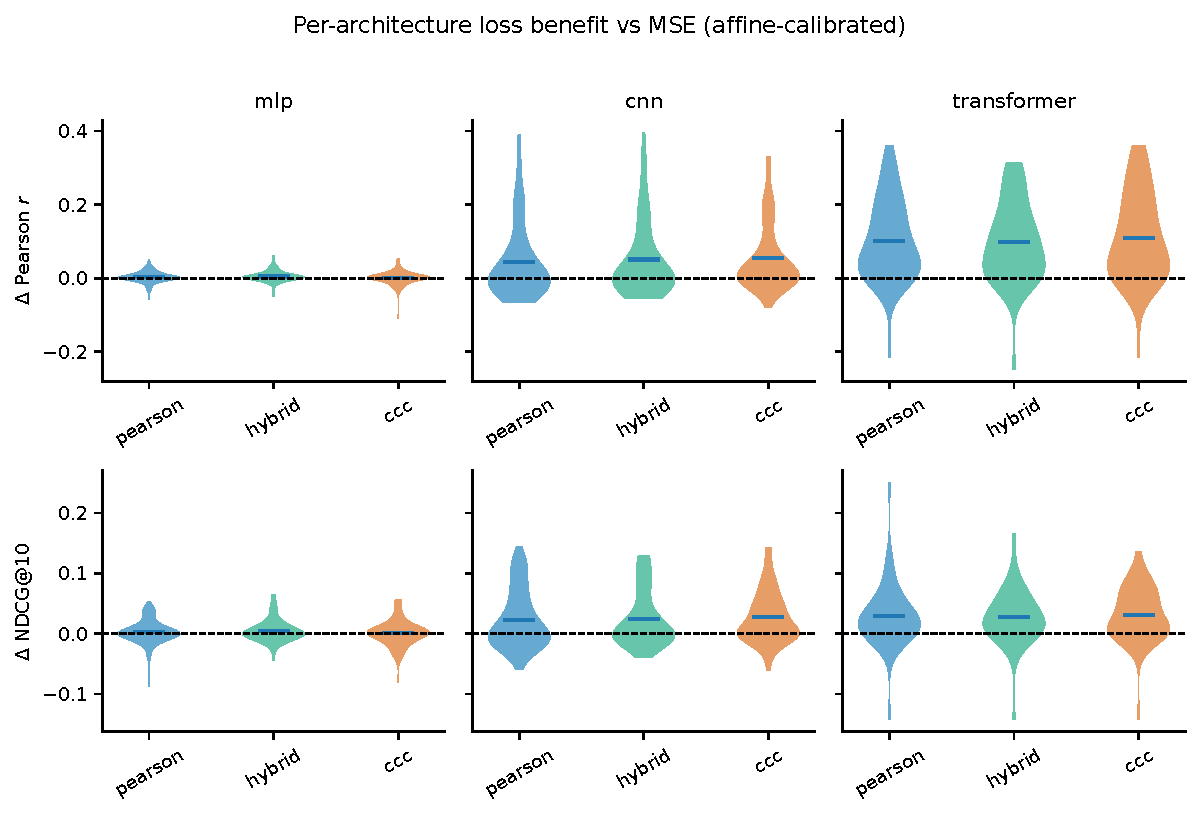
\includegraphics[width=\linewidth]{figS_arch_deltas.pdf}
\caption{Per-architecture distributions of $\Delta$ Pearson $r$ (top) and
$\Delta$ NDCG@10 (bottom) for the Pearson, hybrid and CCC losses relative to MSE,
for the affine-calibrated MLP, CNN and Transformer. Violins show the
distribution over (dataset, trait) cells; the dashed line marks no change. The
benefit is substantial for the CNN and Transformer and small for the well-tuned
MLP.}
\label{fig:S-arch-deltas}
\end{figure}

\begin{figure}[ht]
\centering
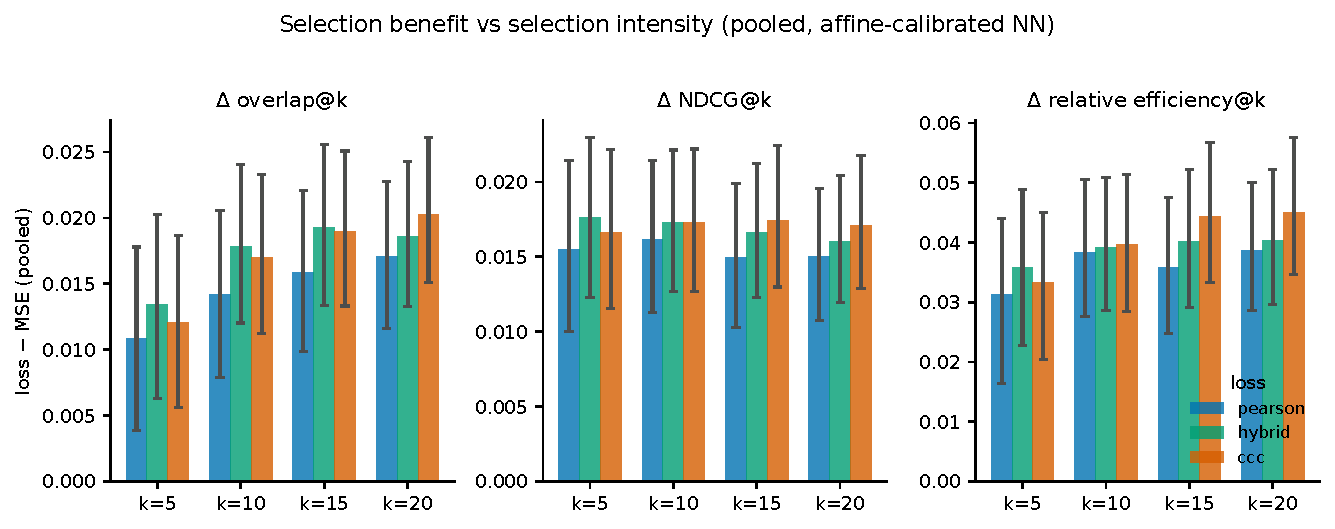
\includegraphics[width=\linewidth]{figS_selection_k.pdf}
\caption{Pooled $\Delta$ of three selection metrics --- top-$k$ overlap, NDCG@k
and relative efficiency@k --- at selection sizes $k\in\{5,10,15,20\}$, for the
affine-calibrated neural network. Bars are bootstrap means with BCa 95\%
confidence intervals; the dashed line marks no change. The selection advantage
of correlation-consistent training is present across selection intensities.}
\label{fig:S-selection-k}
\end{figure}

\begin{figure}[ht]
\centering
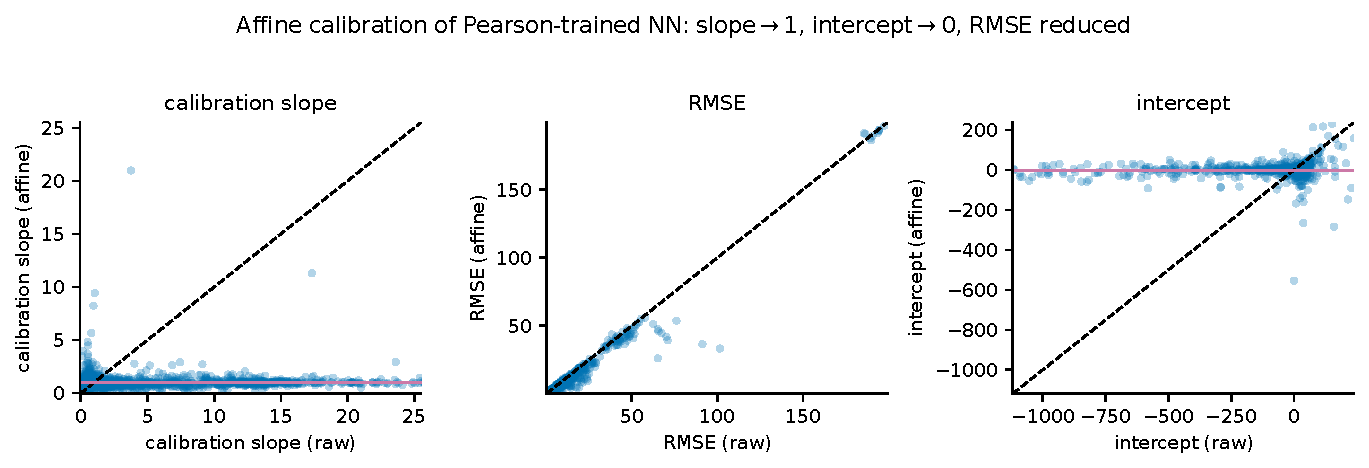
\includegraphics[width=\linewidth]{figS_calibration.pdf}
\caption{Affine calibration of the Pearson-trained neural network (extends main
text Fig.~5). Each point is a cross-validation fold; raw values on the $x$-axis,
affine-calibrated values on the $y$-axis, for the calibration slope, RMSE and
intercept. Calibration drives the slope towards 1 and the intercept towards 0
and reduces RMSE while leaving the rank correlation unchanged.}
\label{fig:S-calibration}
\end{figure}

\begin{figure}[ht]
\centering
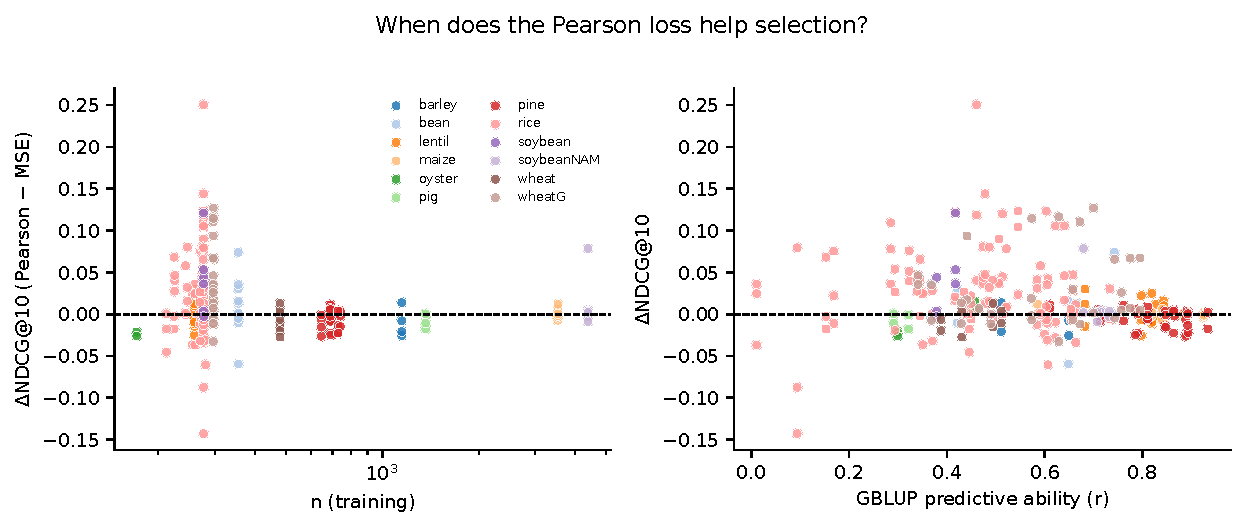
\includegraphics[width=\linewidth]{figS_meta.pdf}
\caption{Meta-analysis of when correlation-consistent training helps selection.
$\Delta$ NDCG@10 of the Pearson loss versus MSE plotted against training-set size
(left) and against GBLUP predictive ability (right), colored by species, for the
affine-calibrated neural network.}
\label{fig:S-meta}
\end{figure}

\begin{figure}[ht]
\centering
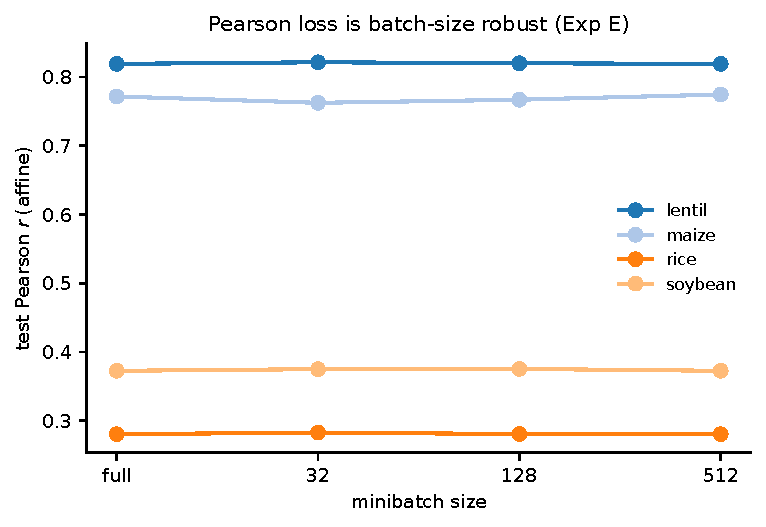
\includegraphics[width=0.75\linewidth]{figS_batch.pdf}
\caption{Experiment E: test Pearson $r$ (affine-calibrated MLP, Pearson loss)
versus minibatch size for each of four EasyGeSe datasets (``full'' = full-batch
gradient). Accuracy is insensitive to the minibatch size.}
\label{fig:S-batch}
\end{figure}

\end{document}
